%%
%% This is file `esapub.tex',
%% generated with the docstrip utility.
%%
%% The original source files were:
%%
%% esapub.dtx  (with options: `manual')
%% ============================================
%% This is the manual describing the usage of
%%      esapub.cls
%% ============================================
%% Copyright 1999 Patrick W Daly
%% Max-Planck-Institut f\"ur Aeronomie
%% Max-Planck-Str. 2
%% D-37191 Katlenburg-Lindau
%% Germany
%% E-mail: daly@linmpi.mpg.de
%%
%% -------------------------------------------------
\documentclass[a4paper,twocolumn]{spaceDebrisC} % European paper
\pagestyle{empty}

\bibliographystyle{plain}

\usepackage{float}

\usepackage{url} % Ensure URLs are properly formatted
\usepackage{xcolor}

% \pagecolor[rgb]{0.0,0.0,0.0}
% \color[rgb]{1,1,1}

\usepackage[section]{placeins} % ensures that floats are placed in their section
\makeatletter
\AtBeginDocument{%
  \expandafter\renewcommand\expandafter\subsection\expandafter{%
    \expandafter\FloatBarrier\subsection
 }%
}
\makeatother

% \makeatletter
% \AtBeginDocument{%
%   \expandafter\renewcommand\expandafter\subsubsection\expandafter{%
%     \expandafter\FloatBarrier\subsubsection
%   }%
% }
% \makeatother

\usepackage{subcaption}
\usepackage{times}
\usepackage[numbers]{natbib}
\usepackage{graphicx}
\usepackage{bm} % for bold math
\usepackage{mathtools} % for \prescript
\usepackage{amssymb}
\usepackage{amsfonts}
\usepackage{adjustbox}

\newcommand{\vctr}[1]{\bm{#1}}
\newcommand{\unitv}[1]{\hat{\vctr{#1}}}
\newcommand{\preup}[1]{\prescript{#1}{}{}}
\newcommand{\rf}[1]{\mathcal{\MakeUppercase{#1}}}
\newcommand{\dcm}[1]{\left[\rf{#1}\right]}
\newcommand{\vrf}[2]{\preup{\rf{#1}}\vctr{#2}}
\newcommand{\mbar}[0]{\;\middle|\;}
\newcommand{\prf}[1]{\preup{\rf{#1}}}
\newcommand{\norm}[1]{\left\lVert#1\right\rVert}

\newcommand{\matcp}[1]{\left[#1 \times\right]}
\newcommand{\rthree}[0]{$\mathbb{R}^3$\:}
\newcommand{\sthree}[0]{$\mathbb{S}^3$\:}
\newcommand{\sothree}[0]{$SO_3$}

\newcommand{\figbig}[0]{0.5\textwidth}
\newcommand{\figmed}[0]{0.4\textwidth}
\newcommand{\figsmall}[0]{0.3\textwidth}

\newcommand{\subfigmed}[0]{0.4\textwidth}
\newcommand{\subfigsm}[0]{0.29\textwidth}
\newcommand{\subfigbig}[0]{0.43\textwidth}

\DeclareMathOperator{\atantwo}{atan2}
\DeclareMathOperator{\fl}{floor}
\DeclareMathOperator*{\argmin}{arg\,min}

\title{Optimal Light Curve Attitude Inversion with Measurement Noise: Two Case Studies}
\author{Liam Robinson}
\author{Carolin Frueh}
\affil{Purdue University, West Lafayette, United States, Email: \texttt{\{robin502, cfrueh\}$@$purdue.edu}}

\begin{document}

\keywords{Light curve inversion; Atitude estimation; Photometry; Inverse problems}

\maketitle

\begin{abstract}

Understanding the orientation and angular velocity state of active or passive human-made space objects is critical for many space situational awareness operations like long-term orbit propagation, anomaly resolution, determining mission status, and active debris removal. Beyond low-Earth orbit, optical telescopes are predominantly used to track space objects. Due to atmospheric distortion and aperture size, it is generally impossible to resolve even large satellites and rocket bodies in optical ground-based imagery. As a result, shape and orientation information is unavailable in individual images, but a measurement of the object's total brightness can still be obtained. Even if the object's shape and reflective properties are known, any given brightness measurement will generally correspond to infinitely many possible orientations. To constrain the solution space, the brightness can be tracked over time -- producing a sequence of measurements called a light curve. If the object's identity is known, its attitude profile can be estimated from the light curve -- up to certain ambiguities -- through a process known as light curve attitude inversion. Due to symmetries in the observation geometry and object shape, there may be multiple attitude profiles that are equally likely to produce any given light curve. Environmental and instrumental measurement noise worsens these ambiguities. To reliably identify these ambiguous solutions, global attitude inversion methods must thoroughly search the solution space.

In this work, we apply a BFGS-based multi-start global attitude inversion algorithm to synthetic observations of an upper stage and real observations taken by the Purdue Optical Ground Station of a Delta I upper stage and the ECHOSTAR II satellite. Given a light curve with an estimate of the shape and reflective properties of the object, our procedure searches the space of initial orientations, angular velocities, and inertia tensors to find initial conditions that produce light curves with low error compared to the observed values. Our formulation inherently accounts for the aforementioned ambiguities, the physical constraints of torque-free rigid body motion, and the noise in the light curve.

\end{abstract}

\section{Introduction}

Knowledge of spacecraft orientation and angular velocity states is critical for many space situational awareness (SSA) tasks. Understanding the evolution of high area-to-mass ratio objects \cite{frueh2014} and decommissioned satellites \cite{rachman2023}, planning and executing active debris removal \cite{bonnal2013}, and recovering from mission anomalies \cite{umansky2023} all require attitude information. 

Methods for estimating the attitude state of uncontrolled space objects from light curves differ significantly depending on the presence of an initial guess. If a guess is available, many filter-based approaches have been developed to process new photometry to update the guess orientation and angular velocity. This class of methods includes single Kalman filters \cite{burton2021two, gagnon2024, wetterer2009}, and multi-filter multiple-model adaptive estimation (MMAE) schemes \cite{linares2014space, dianetti2020}. These approaches can be very effective if the initial state estimate is close to the truth, but have been reported to diverge even in cases when the initial guess guess is within $5^\circ$ of the ground truth orientation and $0.03^\circ/s^{-1}$ in angular velocity error \cite{gagnon2024} due to measurement nonlinearity and ambiguities.

If no initial attitude guess is available, as in most cases of passive debris observation, the inversion problem must be solved globally. Filtering approaches can be applied here too; particle \cite{linares2014particle, holzinger2014} and Bayesian Multi-Hypothesis filters \cite{burton2021two, cabrera2023} have shown promise in prior work, but still rely on high-quality priors as with the Kalman filters. In the absence of prior knowledge about the object's attitude state, simulated annealing \cite{gagnon2024, clark2020}, genetic algorithms \cite{gagnon2024, piergentili2017, clark2020}, and particle swarm optimizers (PSOs) \cite{clark2020, clark2022, burton2024journal, burton2024scitech, gagnon2024} can be applied to search the solution space exhaustively.

While much work has performed full state attitude inversion on simulated light curve data \cite{burton2024journal, gagnon2024, robinson2025att}, studies using real data often focus on determining a constant spin rate and axis of rotation for the observed object.

Frequency analysis in the form of periodograms, Fourier transforms, or epoch folding, is often used to determine the spin rate based on the light curve's frequency spectrum \cite{silha2015, silha2021, isoletta2024, schildknecht2015, pittet2017, yanagisawa2012, koshkin2018}. If optical material properties are known, the width of a single specular glint can provide sufficient information to determine the rotation rate \cite{hinks2016}. There has also been interest in tracking the evolution of spin rates over time for different classes of objects in different orbital regimes \cite{koshkin2018, blacketer2022, karpov2016}. These spin rate determination methods are designed for single-axis rotations and can fail for tumbling objects.

The rotation axis is often estimated for diffusely reflecting objects that are well-approximated as ellipsoids via the so-called amplitude method \cite{williams1979location} which has been extended for combined spin and precession motion \cite{yanagisawa2012}. For light curves with strong specular peaks, the timing of these glints can be used to determine the constant rotation axis given multiple passes of observations \cite{vananti2023, koshkin2018}. These approaches are not applicable for generalized rigid body motion where no simplifying assumptions about the location of the spin axis are available.

The simplifying assumptions of constant, single-axis rotation that are commonly made when working with real data enable elegant solutions, but break down when the observed object is in a complex spin profile. Methods for full attitude state solutions -- time-varying orientation and angular velocities -- have been developed \cite{clark2022, burton2024journal, gagnon2024, linares2014particle}, but are seldom applied to real data. Works that have been successful at estimating a full rigid body attitude state from real data include genetic algorithms \cite{piergentili2020, gallucci2020} and brute-force grid search \cite{shafer2017}. Any full-state estimation method must tackle the inherent computational complexity, lack of knowledge of material reflectivities, and the presence of measurement noise.

In this paper, we describe a global full-state attitude solver inspired by recent PSO work \cite{burton2024journal} but is easier to tune, can be fully parallelized, and is robust to significant measurement noise \cite{robinson2025att}. Further, our method differs from other global estimation methods in that we do not seek to find one optimal solution and instead search for a collection of high-quality local minima to directly study the many ambiguous solutions for a given light curve. Our approach was designed specifically for use with real data as we take time-varying measurement noise and uncertainties in the body moments of inertia into account explicitly. 

To solve the optimization problem, we sample many candidate solutions scattered throughout the solution space and perform gradient-based optimization on each using the BFGS algorithm. Our optimization procedure reliably converges to high-quality maximum likelihood estimates of the attitude state. The final output of our method is an array of the best solutions, ranked by their likelihood. Clusters of low-error minima can be analyzed to identify families of solutions.

This work proceeds by describing the inversion method, discussing efficient methods for computing the time-varying probability density of the light curve. We present inversion results for a simulated rocket body light curve where the ground truth is known, followed by two cases -- a derelict satellite and rocket body -- using real light curve data collected by the Purdue Optical Ground Station. A deeper treatment of our method and additional simulated light curve results can be found in \cite{robinson2025att}.

\section{Inversion Method}

\subsection{State Definition and Dynamics}

The state vector $\vctr{x}$ is defined to be the concatenation of the Modified Rodriguez Parameter (MRP) $\vctr{p} = [p_1, p_2, p_3]^T$, the principal body frame angular velocity $\vctr{\omega} = [\omega_1, \omega_2, \omega_3]$ in radians per second, and the ratios of the principal moments of inertia $J_y / J_x$ and $J_z / J_x$ where the constant inertia tensor in principal axes is $J = \mathrm{diag}\left([J_x, J_y, J_z]\right)$:

\begin{equation}
 \vctr{x} = \begin{bmatrix} 
 p_1 & p_2 & p_3 & \omega_1 & \omega_2 & \omega_3 & J_y / J_x & J_z / J_x
  \end{bmatrix}^T.
\end{equation}

The first six elements of the state vector are time-varying with dynamics given by:

\begin{align}
 \vctr{\dot{p}} &= \frac{1}{4} \left[ \left(1 - \vctr{p} \cdot \vctr{p}\right) + 2\vctr{p} \times \vctr{\omega} + 2 \left(\vctr{\omega} \cdot \vctr{p} \right)\vctr{p} \right], \label{eq:mrp_kde} \\
 \vctr{\dot{\omega}} &= J^{-1} \left[ \left(J \vctr{\omega}\right) \times \vctr{\omega} + \vctr{M}\right]. \label{eq:rbtf_dynamics}
\end{align}

\subsection{Objective Function}

Our inversion method is based on the global minimization of a maximum-likelihood loss function which computes the negative log-likelihood of the observed light curve $\vctr{S}$ being a sample from the normal distribution defined by the estimated light curve mean $\hat{\vctr{S}}$ and the standard deviation at each $k$th timestep $\sigma_k$:

\begin{equation} \label{eq:nll_loss}
 f(\vctr{x}) = \frac{1}{m}\sum_{k=1}^{m}\left[\ln\sigma_k + \frac{1}{2}\left(\frac{\vctr{S}_k - \hat{\vctr{S}}_k(\vctr{x})}{\sigma_k}\right)^2 \right].
 \end{equation}

If the reflectivity of the object's faces is not well-known, we rescale the estimated light curve mean $\hat{S}(\vctr{x})$ to have equal $\ell_2$ norm to the observations to resolve the inherent albedo-area ambiguity:

\begin{equation}
 \hat{S}(\vctr{x}) = \frac{\norm{S}}{\norm{\tilde{S}(\vctr{x})}} \tilde{S}(\vctr{x}),
\end{equation}

\noindent
where $\tilde{S}(\vctr{x})$ is the original, poorly scaled, estimated light curve. In this work, the light curve and its standard deviation are always assumed to be expressed in a linear unit, e.g., analog-to-digital units (ADU) or irradiance proportional to $W/m^2$.

\subsection{Computing Local Minima} \label{sec:run_solver}

Our multi-start solution method begins by creating $n$ guesses scattered throughout the solution space -- possibly sampled from a prior distribution based on available knowledge. In the most basic case, the initial state guess is sampled for guess $i$ at iteration $k=0$:

\begin{equation}
 \vctr{x}_{0,i}(0) = \begin{bmatrix}\vctr{p}_{i,0}(0) & \vctr{\omega}_{i,0}(0) & \left(J_y / J_x\right)_{i,0} & \left(J_z / J_x\right)_{i,0}\end{bmatrix}^T.
\end{equation}

\noindent
In this work, $\vctr{p}_{i,0}(0)$ is uniformly randomly sampled from orientation space, $\vctr{\omega}_{i,0}(0)$ is uniformly randomly sampled from the ball in $\mathbb{R}^3$ of radius $\norm{\vctr{\omega}}_\text{max}$ -- the maximum angular rate at which to initialize guesses -- while $\left(J_y / J_x\right)_{i,0}$ and $\left(J_z / J_x\right)_{i,0}$ are sampled from Gaussian prior distributions centered at estimated values derived from the known geometry of the object. We determine $\norm{\vctr{\omega}}_\text{max}$ based on the maximum power positive frequency in the observed light curve $f^\star$ in Hertz and an arbitrary safety factor $f_\omega \geq 1$, selected as $f_\omega = 1.25$ for this work:

\begin{equation} \label{eq:ang_vel_max}
  \norm{\vctr{\omega}}_\text{max} = 2\pi f_\omega f^\star.
\end{equation}

Even for a well-chosen bound $\norm{\vctr{\omega}}_\text{max}$, there may still be numerous high-quality solutions at significantly lower or higher angular velocities that possess equal $f^\star$ values due to object shape symmetries or harmonics in spin and precession rates, respectively. As a result, it is usually unwise to directly constrain the angular velocity to a given magnitude unless additional, unambiguous information is available.

After computing each initial state guess, we run the Broyden-Fletcher-Goldfarb-Shanno (BFGS) algorithm \cite{broyden1970, fletcher1970, goldfarb1970, shanno1970} to optimize each guess to a nearby local minimum $\vctr{x}_{k,i}(0)$ in the objective function such that:

\begin{equation} \label{eq:opt_problem}
 \vctr{x}_{k,i}(0) = \argmin_{\vctr{x}} f(\vctr{x}),
\end{equation}

\noindent
producing a final initial state which is a good local guess for a state that produces the observations. In this way, we globally search the solution space up to the density implied by $n$. Using a simpler algorithm like gradient descent can still reach convergence, but will take significantly more objective function evaluations due to the high nonlinearity of the attitude inversion problem.

In order to implement this optimization effectively without constraints, it is often necessary to take the absolute value of the intermediate inertia tensor values to maintain physical validity. 

\subsection{Classifying Candidate Solutions} \label{sec:candidate_sols}

Although all initial conditions will converge to some nearby local minimum, many of these minima will possess a low likelihood determined by $-\mathrm{exp}(f(\vctr{x}))$. As we do not generally know how large the geometric and material mismatch between the observed object and the assumed model is, we cannot put a strict bound on a likelihood level that constitutes a high-quality candidate solution. In this work, we identify candidate solutions by choosing a likelihood ratio tolerance $0 < \ell < 1$, such that all solutions $\vctr{x}_{i,k}(0)$ are candidates for the truth if:

\begin{equation}
  e^{-f(\vctr(x)_{i,k}(0))} > \ell e^{-f(\vctr(x)^\star_{k}(0))}.
\end{equation}

Here, $\vctr(x)^\star_{k}(0) = \argmin_{\vctr{x}_{i,k}(0)} f(\vctr(x)_{i,k}(0)) $ is the highest likelihood solution found after optimization.

\section{Computing the Light Curve}

\subsection{Object Geometry Definition}

We choose to represent the surface geometry of space objects as a polyhedral mesh composed of a collection of flat facets. Each $i$th face has $n_v \geq 3$ or more vertices $\left\{ v_{i,1}, v_{i,2}, v_{i,n_v} \right\}$ and an outward-pointing normal vector $\unitv{n}_i$. The total facet area is computed for an arbitrary planar polygon via:

\begin{equation} \label{eq:poly_area}
 A(P) = \sum_{j=0}^{k-3} \frac{\| \left( \vctr{v}_{j+1} - \vctr{v}_{j} \right) \times \left( \vctr{v}_{j+2} - \vctr{v}_{j} \right)\|_2}{2}.
 \end{equation} 
 
 In any particular illumination and observation condition, a fraction of the facet's area $\tilde{a}_i$ may be Sun- or observer-shadowed due to obstructing geometry before or after light reaches the surface element, respectively. The remainder of the facet's area $\bar{a}_i$ is unshadowed and contributes to the total flux reaching the observer from the object, such that the total area of each facet is $a_i = \tilde{a}_i + \bar{a}_i$. The geometry for an individual facet is displayed in Figure \ref{fig:facet_geom}.

\begin{figure}[H]
  \centering
  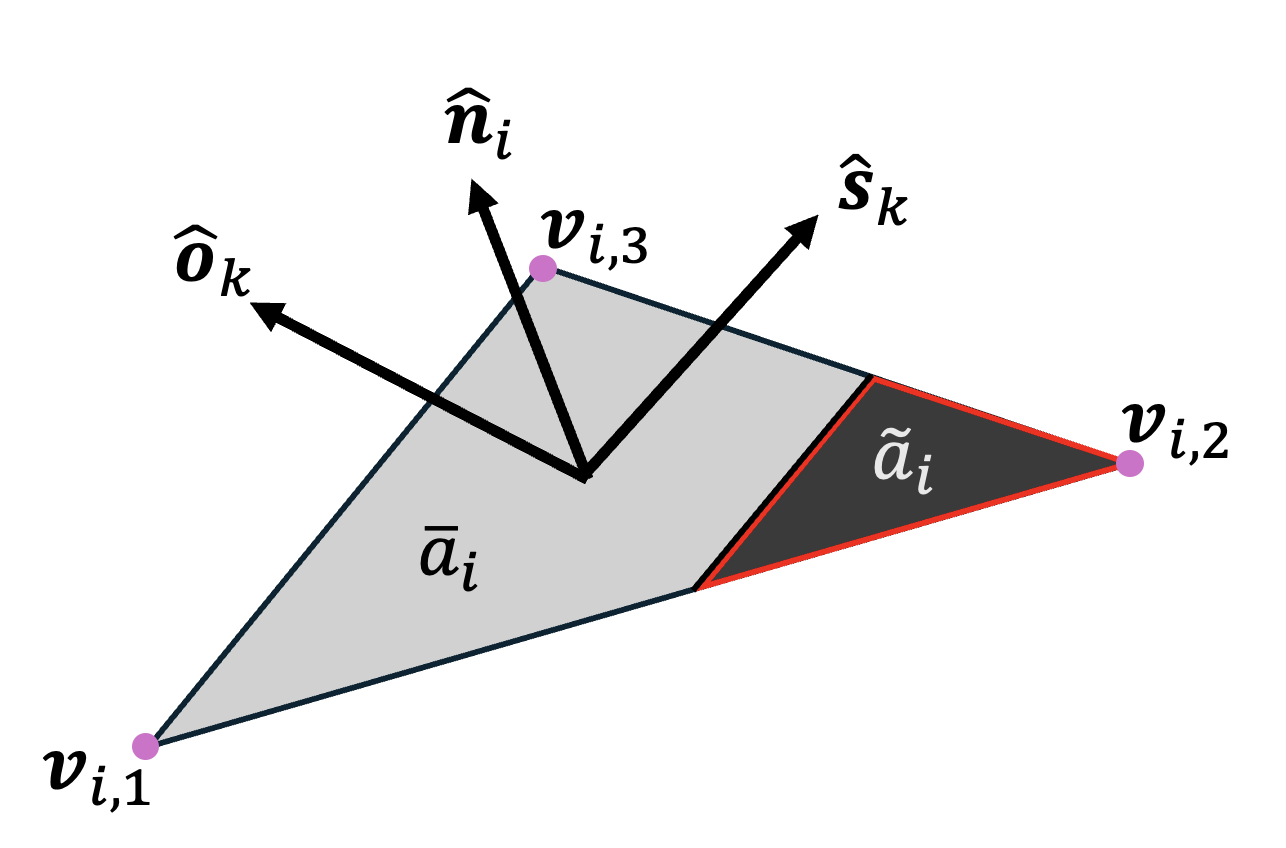
\includegraphics[width=\figmed]{obs_geom.png}
  \caption{Facet geometry including the observer direction $\unitv{o}$, Sun direction $\unitv{s}$, normal vector $\unitv{n}_i$, unshadowed area $\bar{a}_i$, shadowed area $\tilde{a}_i$, and counterclockwise vertex positions $\left\{ \vctr{v}_{i,1}, \vctr{v}_{i,2}, \vctr{v}_{i,3} \right\}$.}
  \label{fig:facet_geom}
\end{figure}

In this work, the Sun position is computed using a SPICE ephemeris kernel \cite{spice} while space object positions are propagated with SGP4 TLEs obtained from Space-Track \cite{spacetrack}.

\subsection{Computing the Unshadowed Area}

The unshadowed area $\bar{a}$ may be computed in several ways. For convex objects, $\bar{a}=a$ as self-shadowing is impossible. For highly nonconvex and detailed models composed of thousands of faces, $\bar{a}$ can be approximated on a pixel grid using shadow mapping \cite{robinson2022}. Self-shadowing can be efficiently solved semi-analytically for lower-fidelity approximations of real space object geometry by computing the mutual intersections of the polygons $P_k$ of other faces whose projections overlap with the face in question. Up to a maximum intersection depth $d$, selected for computation time, the unshadowed area can be computed via:

\begin{equation} \label{eq:us_area}
 \bar{a} = a - \sum_{d=1}^{n} \sum_{K \in \text{comb}(n,d)} (-1)^{d+1} A\left(\bigcap\limits_{k \in K} P_k\right).
\end{equation}

As the objects we investigate in this work are well-approximated with relatively simple non-convex meshes, we use the semi-analytic method to efficiently compute unshadowed areas via the Sutherland-Hodgeman algorithm \cite{sutherland1974} for each polygon intersection. Further explanation of the polygon clipping procedure for computing the total shadowed area and accelerating this computation during inversion with the so-called shadow cache is included here \textbf{TODO: should this be a here? wording this felt weird if we're avoiding saying like "the authors'"} \cite{robinson2025att}.

\subsection{Surface Reflectivity}

The bidirectional reflectance distribution function (BRDF) defines the amount of incident radiation from $\unitv{s}$ reflected per steradian in the observer's direction $\unitv{o}$. We choose the Blinn-Phong \cite{blinn1977} BRDF for this work as it is efficient to compute and satisfies the three main requirements for a physically meaningful BRDF as it is nonnegative, energy-conserving, and reciprocal \cite{duvenhage2013}. We avoid microfacet models for computational efficiency, and because in practice, the uncertainty in the reflective properties of the observed objects will often be larger than errors introduced by the choice of reflection model. The Blinn-Phong BRDF is parameterized by the coefficient of diffuse reflectivity $C_d$, the coefficient of specular reflectivity $C_s$, and the specular exponent $n>0$ \cite{duvenhage2013}:

\begin{equation} \label{eq:brdf_blinn_phong}
 f_r(\unitv{s}, \unitv{o}) = \frac{C_d}{\pi} + \frac{n+2}{2\pi} \frac{C_s (\unitv{n} \cdot \unitv{h})^n}{4 (\unitv{n} \cdot \unitv{s})(\unitv{n} \cdot \unitv{o})}.
\end{equation}

The coefficients of reflectivity implicity satisfy $C_a + C_s + C_d = 1$ for energy conservation, where $ 0 \leq C_a \leq 1$ is the coefficient of absorption \cite{fan2020thesis}.

Here, the halfway vector $\unitv{h}$ bisects the illumination and observation directions such that $\unitv{h} = \unitv{h} = (\unitv{s} + \unitv{o})/\norm{\unitv{s} + \unitv{o}}$ \cite{duvenhage2013}.

\subsection{Computing the Mean Observed Signal}

Given the observer $\unitv{o}_k$ and illumination directions $\unitv{s}_k$ at the $k$th observation epoch in the body frame $\mathcal{B}$, as well as the BRDF $f_{r,i}$ for each $i$th surface of the object, the fraction of incident power reflected in the direction of the observer is \cite{fan2020thesis}:

\begin{equation} \label{eq:lc_norm}
  \begin{split} 
 f_p(\unitv{s}_k, \unitv{o}_k) = \sum_{i=1}^n\prf{B}[&\bar{a}_i(\unitv{s}_k, \unitv{o}_k) f_{r,i}(\unitv{s}_k, \unitv{o}_k) \\ \cdot &(\unitv{n}_i \cdot \unitv{s}_k) (\unitv{n}_i \cdot \unitv{o}_k)]. 
  \end{split} 
\end{equation}

The output of Equation \ref{eq:lc_norm} is a light curve, but as many of the noise characteristics of the signal are defined in the image sensor's native unit of ADU, we convert the light curve into the same units via:

\begin{equation} \label{eq:general_bright}
  \begin{split} 
 \bar{S}_{\text{SO},k} = &f_p(\unitv{s}_k, \unitv{o}_k) \frac{A_\circ \Delta t_k f_\odot(\vctr{r})}{g R_\oplus^2 r_k^2} \\ \cdot &\int_{0}^{\infty}{P(\lambda)Q(\lambda)T_k(\lambda) I_\odot(\lambda) \left(\frac{\lambda}{hc}\right)}\,d\lambda. 
  \end{split}
\end{equation}

Here before the integral, $A_\circ$ is the unobstructed aperture area in square meters, $\Delta t_k$ is the exposure time in seconds, $f_\odot(\vctr{r})$ is the fraction of solar irradiance reaching the space object at position $\vctr{r}$ -- accounting for the Earth's shadow, $g$ is the sensor gain in ADU per photoelectron, $R_\oplus$ is the distance from the Sun to the space object in AU, $r_k$ is the distance from the observer to the space object in kilometers. Within the integral, we account for the telescope's passband filter $P(\lambda)$, the image sensor quantum efficiency $Q(\lambda)$, the atmospheric absorption spectrum $T_k(\lambda)$, the solar irradiance spectrum $I_\odot(\lambda)$, and the inverse energy of a photon with wavelength $\lambda$, $\lambda / hc$, where $h$ is Planck's constant in Joule-seconds, and $c$ is the speed of light in vacuum in meters per second. Taken together, the integral computes the fraction of the energy reflected from the object absorbed into the image sensor, while the outer factor dimensionalizes the result to yield the mean total sensor response in ADU across all pixels due to the object's signal.

\subsection{Approximating the Measurement Noise}

This section summarizes an in-depth study of relevant noise sources in CCD and CMOS sensor light curves which can be found in \cite{robinson2025twin}.

The variance of a space object's observed brightness whose mean is determined by Equation \ref{eq:general_bright} is a combination of many independent stochastic processes. These distributions have variances $\sigma^2_\text{sensor}$ due to the sensor's integration and readout effects, $\sigma^2_\text{flat}$ from sensor flat-fielding effects, scintillation noise $\bar{S}_{\text{SO},k} \sigma^2_{Y,k}$ \cite{osborn2015}, Poisson signal shot noise $\lambda_{\text{shot},k}$, and Poisson background noise $\lambda_{\text{back},k}$. The sum of these variances yields the total signal variance in ADU:

\begin{equation} \label{eq:sigma_total}
  \begin{split}
  \sigma^2_{S,k} = &\lambda_{\text{back},k} + \bar{S}_{\text{SO},k} \sigma^2_{Y,k} + \lambda_{\text{shot},k} \\ + &\sigma^2_\text{flat} + \sigma^2_\text{sensor}.
  \end{split}
\end{equation}

The sensor noise is approximated by the independent combination of Poisson dark current $\lambda_\text{dark}$ and readout noise $\sigma_\text{read}^2$ \cite{krag2003}:

\begin{equation} \label{eq:sensor_noise}
  \sigma_\text{sensor}^2 = n_\text{pix} \left( \Delta t \cdot \lambda_\text{dark} + \sigma_\text{read}^2 \right).
\end{equation}

The flat field noise is modeled as a zero-mean Gaussian linearly scaling with the signal in each of the $n_\text{pix}$ pixels of the object signal $S_i$ and a constant $f_k$ fit to the sensor from flat frame observations, yielding the signal standard deviation \cite{newberry1996}: 

\begin{equation}
  \sigma_\text{flat}^2 = f_k^2 \sum_{i=1}^{n_\text{pix}} S_i^2.
\end{equation}

The background standard deviation is modeled by the sum of six independent Poisson random processes contributing to light entering the telescope optics from environmental sources. These processes and the sources of their respective models are: scattered moonlight $\lambda_{\text{moon},k}$ \cite{daniels1977}, integrated starlight $\lambda_{\text{star},k}$ \cite{krag2003}, twilight $\lambda_{\text{twi},k}$ \cite{patat2006}, zodiacal light $\lambda_{\text{zod},k}$ \cite{roach1972}, airglow $\lambda_{\text{air},k}$ \cite{krag2003}, and light pollution $\lambda_{\text{poll},k}$ \cite{falchi2016, falchi2016_data}. In summation, the total Poisson background variance is:

\begin{equation}
  \begin{split}
  \lambda_{\text{back},k} = n_{\text{pix},k} ( &\lambda_{\text{moon},k} + \lambda_{\text{star},k} + \lambda_{\text{twi},k} \\+ &\lambda_{\text{zod},k} + \lambda_{\text{air},k} + \lambda_{\text{poll},k} ).
  \end{split}
\end{equation}

The fractional scintillation noise due to atmospheric turbulence is modeled via Young's approximation \cite{osborn2015}:

\begin{equation} \label{eq:scint_noise}
  \sigma^2_{Y,k} = 10^{-6} D^{-4/3} (\Delta t)_k^{-1} \cos^{-3}\left(\gamma_k\right) e^{\frac{-2h_\text{obs}}{H}}.
\end{equation}

Here, the scintillation noise at timestep $k$ as a function of the aperture diameter $D$ in meters, the exposure time $(\Delta t)_k$ in seconds, the zenith angle $\gamma_k$, the observing station's altitude $h_\text{obs}$ in meters, and the turbulence scaleheight $H\approx8000$ meters \cite{osborn2015}.

The signal shot noise is a Poisson process as a function of the mean signal in ADU $\bar{S}_{\text{SO},k}$ and the image sensor gain $g$ in ADU per photoelectron:

\begin{equation}
  \lambda_{\text{shot},k} = \frac{\bar{S}_{\text{SO},k}}{\sqrt{g}}.
\end{equation}

After summation in Equation \ref{eq:sigma_total}, we can approximate the observed light curve as Gaussian distributed via the mean $\bar{S}_{\text{SO},k}$ from Equation \ref{eq:general_bright} and the variance $\sigma^2_{S,k}$ in $\text{ADU}^2$:

\begin{equation} \label{eq:lc_dist}
 S_{\text{SO},k} \sim \mathcal{N}\left( \bar{S}_{\text{SO},k}, \sigma^2_{S,k} \right).
 \end{equation}

\section{Attitude Inversion Results for Synthetic Data}

\subsection{Generating the Observed Light Curve}


To demonstrate the effectiveness of our inversion method, we first present results for a simulated light curve where the ground truth is known. In order to make this simulated case realistic, we use the presented measurement noise models and introduce a mismatch between the ground truth object used to generate the measurements and the model used in inversion. We produce a noisy, observed light curve for a high-fidelity model of the Saturn V second stage scaled down by a factor $10/3$ to act as a template rocket body object, shown on the right of Figure \ref{fig:rb_models}.

% \begin{figure}[H]
%   \centering
%   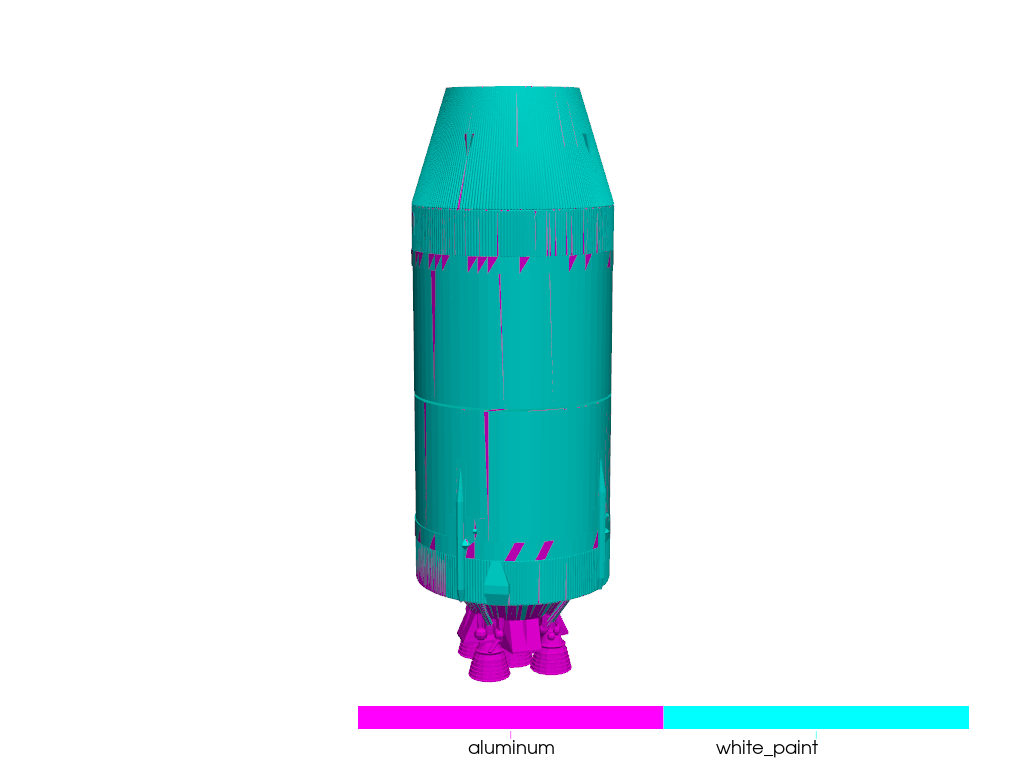
\includegraphics[width=\figsmall]{rocket_bodies2.png}
%   \caption{Simulated truth rocket body model \cite{nasa_models}.}
%   \label{fig:meas_model}
% \end{figure}

Table \ref{tb:case1_in} describes the simulated observation scenario, placing the rocket body in the orbit of an SL-12 upper stage in geosynchronous orbit, observed by the Purdue Optical Ground Station. Relevant geographical and optical properties of this ground station are provided in the Appendix in Table \ref{tb:tele_info}. Table \ref{tb:synth_matprops} lists the material properties used in this test case.

\begin{table}[H]
  \centering
  \caption{Simulated observation characteristics}
  \vspace*{6pt}
  \begin{tabular}{|l|l|}
  \hline
  \textbf{Variable} & \textbf{Value} \\ \hline
 Target COSPAR ID & 1990-054D \\ \hline
 First obs.\ (UTC) & Mar 8, 2025 02:00:00.000 \\ \hline
 Light curve duration & $5$ minutes \\ \hline
 Observations & $100$ \\ \hline
 Integration time & $0.5$ seconds \\ \hline
  \end{tabular}
  \label{tb:case1_in}
\end{table}

\begin{table}[H]
  \centering
  \caption{Reflection properties of materials used in the synthetic data test case. The white paint parameters were estimated qualitatively}
  \vspace*{6pt}
  \begin{tabular}{|l|l|l|l|}
  \hline
  \textbf{Material} & $C_d$ & $C_s$ & $n$ \\ \hline
 Aluminum \cite{fankhauser2023} & $0.34$ & $0.40$ & $8.9$ \\ \hline
 White paint & $0.9$ & $0.1$ & $1$ \\ \hline
  \end{tabular}
  \label{tb:synth_matprops}
\end{table}

The ground truth attitude profile and inertia tensor ratios of the simulated object are listed in Table \ref{tb:synth_att}.

\begin{table}[H]
  \centering
  \caption{True object attitude profile for all test cases}
  \vspace*{6pt}
  \begin{tabular}{|l|l|}
  \hline
  \textbf{Variable} & \textbf{Value} \\ \hline
 Initial $\vctr{p}(0)$ & $-\frac{1}{3} \begin{bmatrix} 1 & 1 & 1 \end{bmatrix}^T$ \\ \hline
 True $\vctr{\omega}(0)$ ($\text{rad}/\text{s}$) & $\vctr{\omega}(0) = \begin{bmatrix} 0.03 & 0.06 & 0.03 \end{bmatrix}^T$ \\ \hline
 Inertia tensor ratios & $J_y / J_x = 1, \: J_z / J_x = 0.25$ \\ \hline
 External torque $\vctr{M}$ & $\begin{bmatrix} 0 & 0 & 0 \end{bmatrix}^T$ \\ \hline
  \end{tabular}
  \label{tb:synth_att}
\end{table}
\FloatBarrier

Simulating the mean light curve and its approximate probability distribution via Equation \ref{eq:lc_dist} produces the light curve displayed in V-band magnitude in Figure \ref{fig:obs_mag_synth}.

% \begin{figure}[H]
%   \centering
%   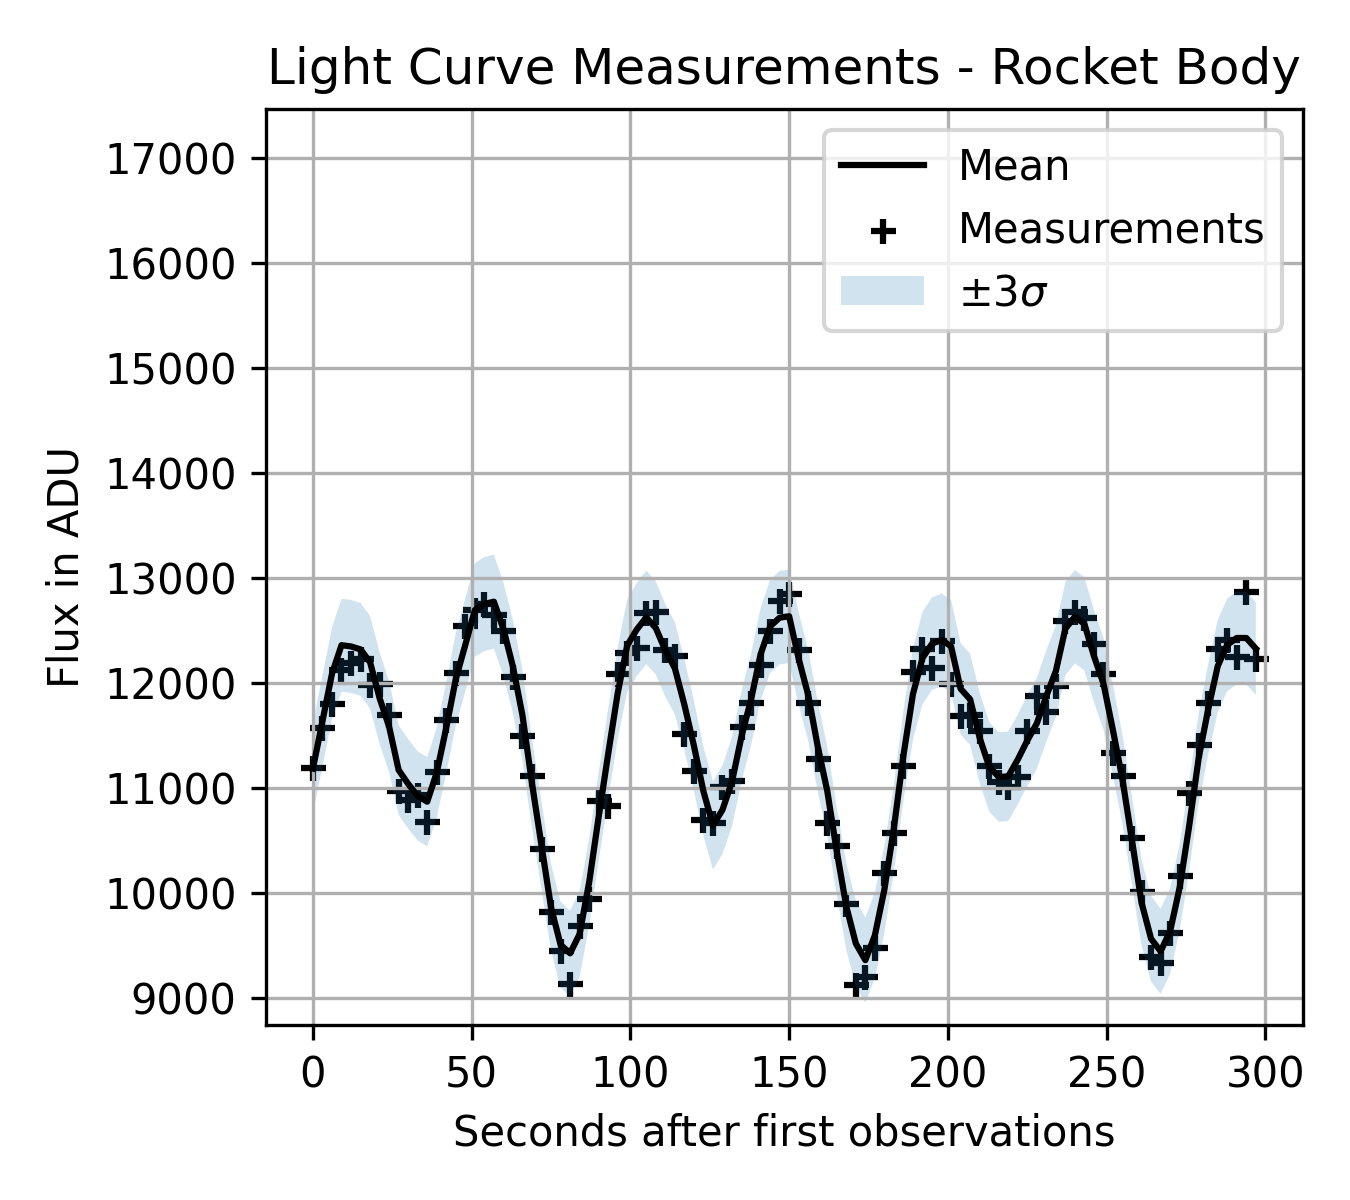
\includegraphics[width=\figmed]{light_curves_adu_rocket_body_sdc.png}
%   \caption{Simulated observed flux for the rocket body.}
%   \label{fig:obs_adu_synth}
% \end{figure}

\begin{figure}[H]
  \centering
  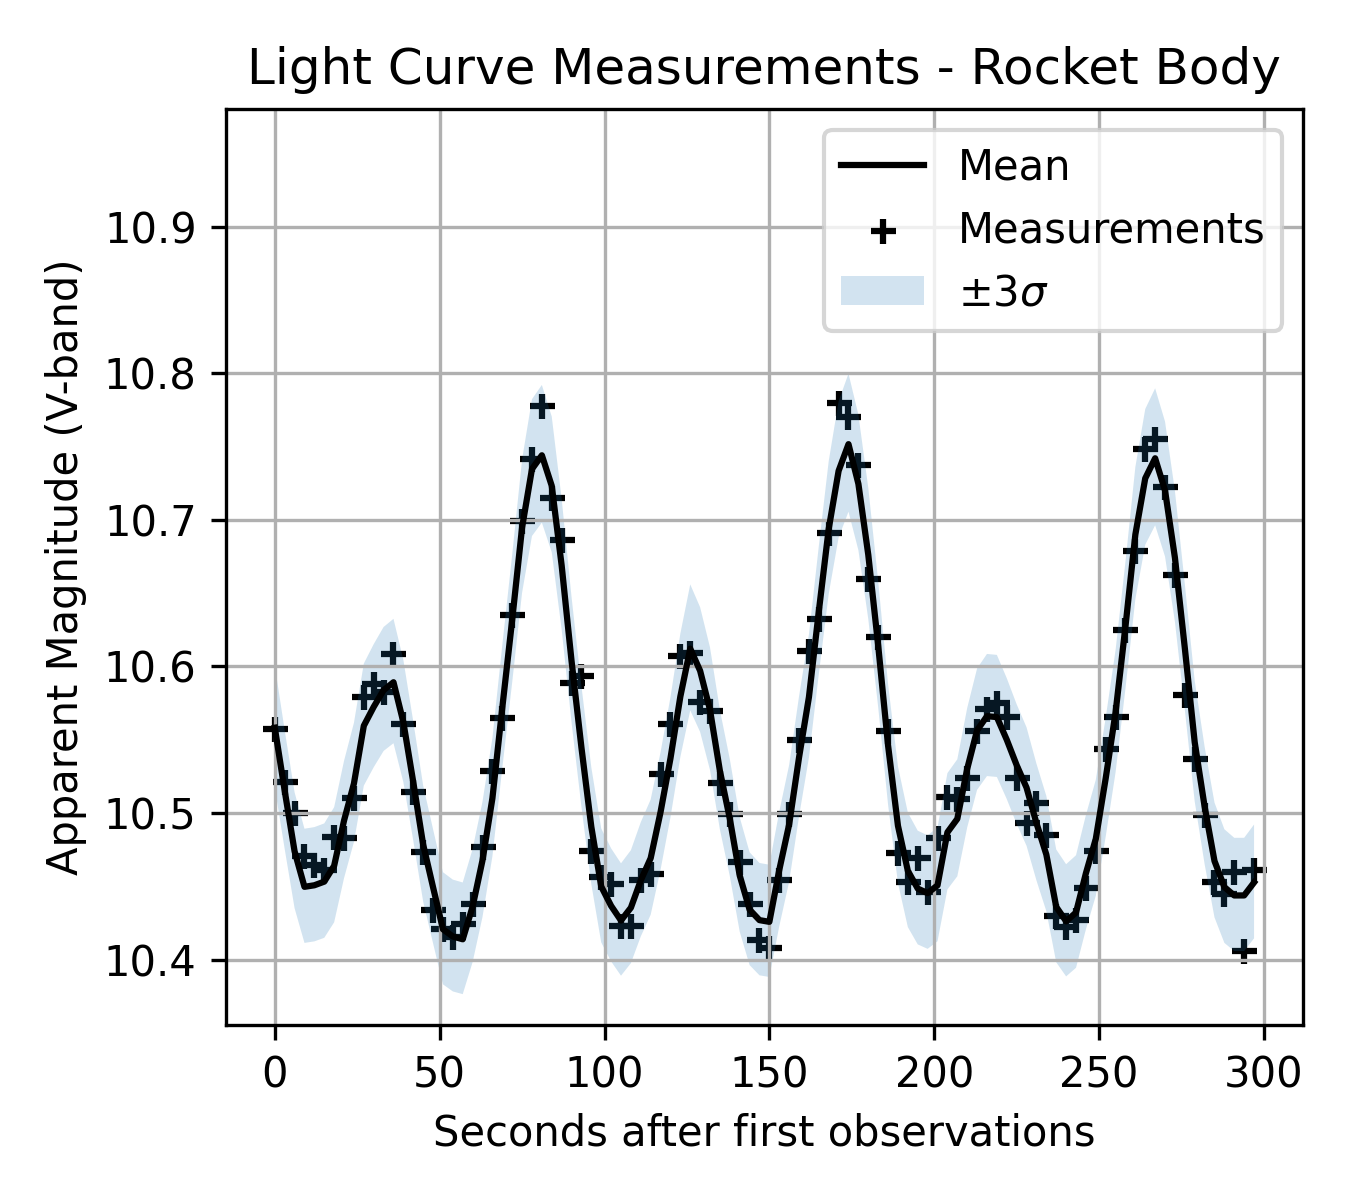
\includegraphics[width=\figmed]{light_curves_mag_rocket_body_sdc.png}
  \caption{Simulated mean and sampled observations for the rocket body in V-band magnitude, with the variance included in blue.}
  \label{fig:obs_mag_synth}
\end{figure}

% \begin{figure}[H]
%   \centering
%   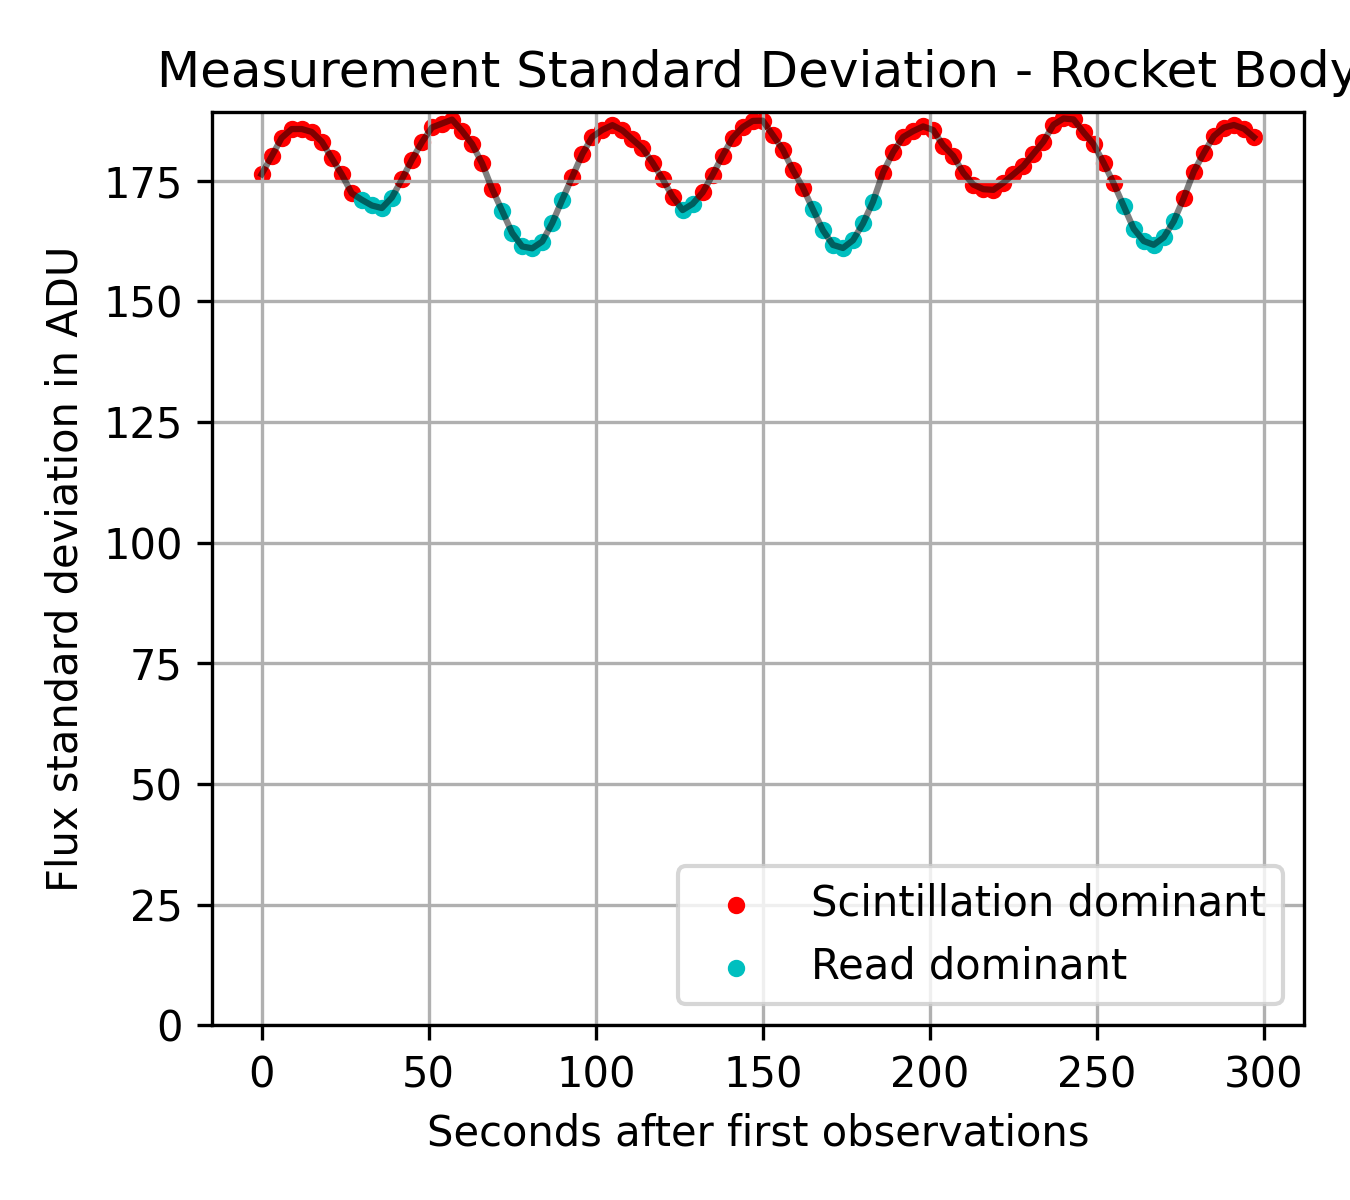
\includegraphics[width=\figsmall]{light_curves_std_rocket_body_sdc.png}
%   \caption{Simulated observed light curve standard deviation computed with Equation \ref{eq:sigma_total}.}
%   \label{fig:obs_std_synth}
% \end{figure}

\subsection{Synthetic Light Curve Optimization Results}

To emulate the reality that the precise geometry of the observed object is usually uncertain, we use perform attitude inversion with a significantly simplified rocket body model, shown in Figure \ref{fig:rb_models}.

\begin{figure}[H]
  \centering
  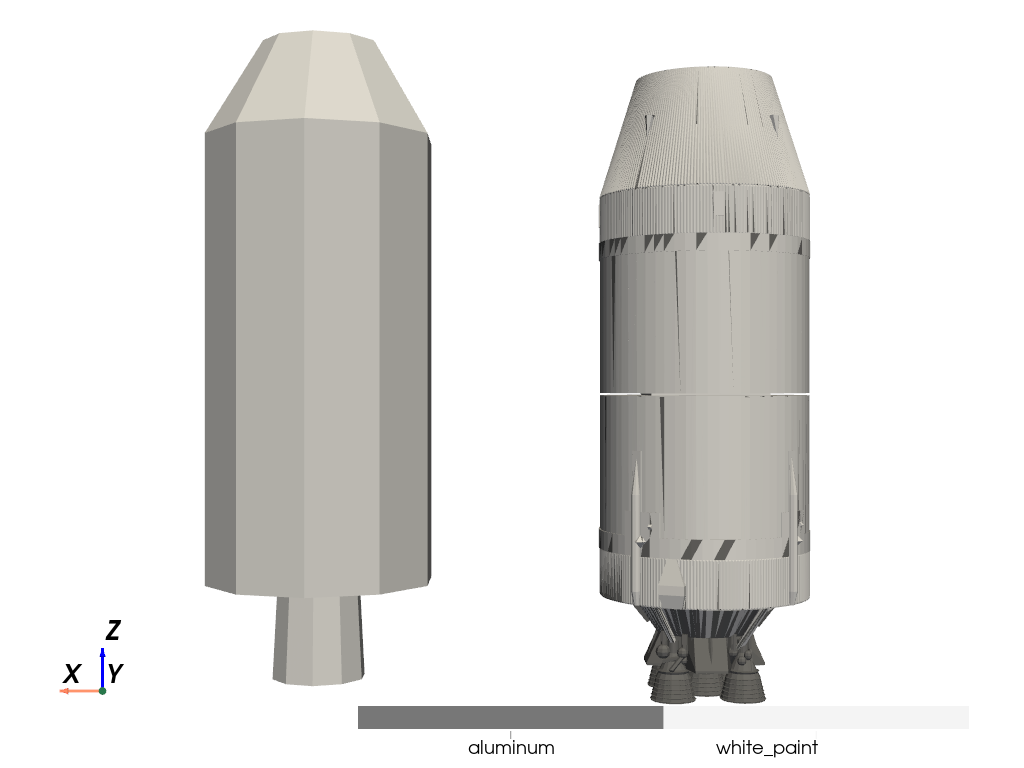
\includegraphics[width=\figmed]{rocket_bodies.png}
  \caption{Simplified rocket body model used for inversion (left) and simulated ground truth model (right).}
  \label{fig:rb_models}
\end{figure}

A total of $10^5$ initial state guesses are created via the sampling scheme described in Section \ref{sec:run_solver} with $\norm{\vctr{\omega}}_\text{max}=5.26$ degrees per second. The inertia tensor ratios are initialized by sampling a symmetric Gaussian distribution with $\sigma=0.05 \: [kg\cdot m^2]$ on each axis to simulate a moderate level of inertia uncertainty. BFGS minimization is then performed for each initial guess to locally solve the optimization problem given by Equation \ref{eq:opt_problem}. Classifying candidate solutions with $\ell = 1/10$ produces over $10^4$ solutions within this bound. Figure \ref{fig:conv_lcs_synth} shows the mean light curves produced by the identified candidate solutions. There is good agreement between the candidate light curves and the observations, indicating that high-quality local minima have been identified.

\begin{figure}[H]
  \centering
  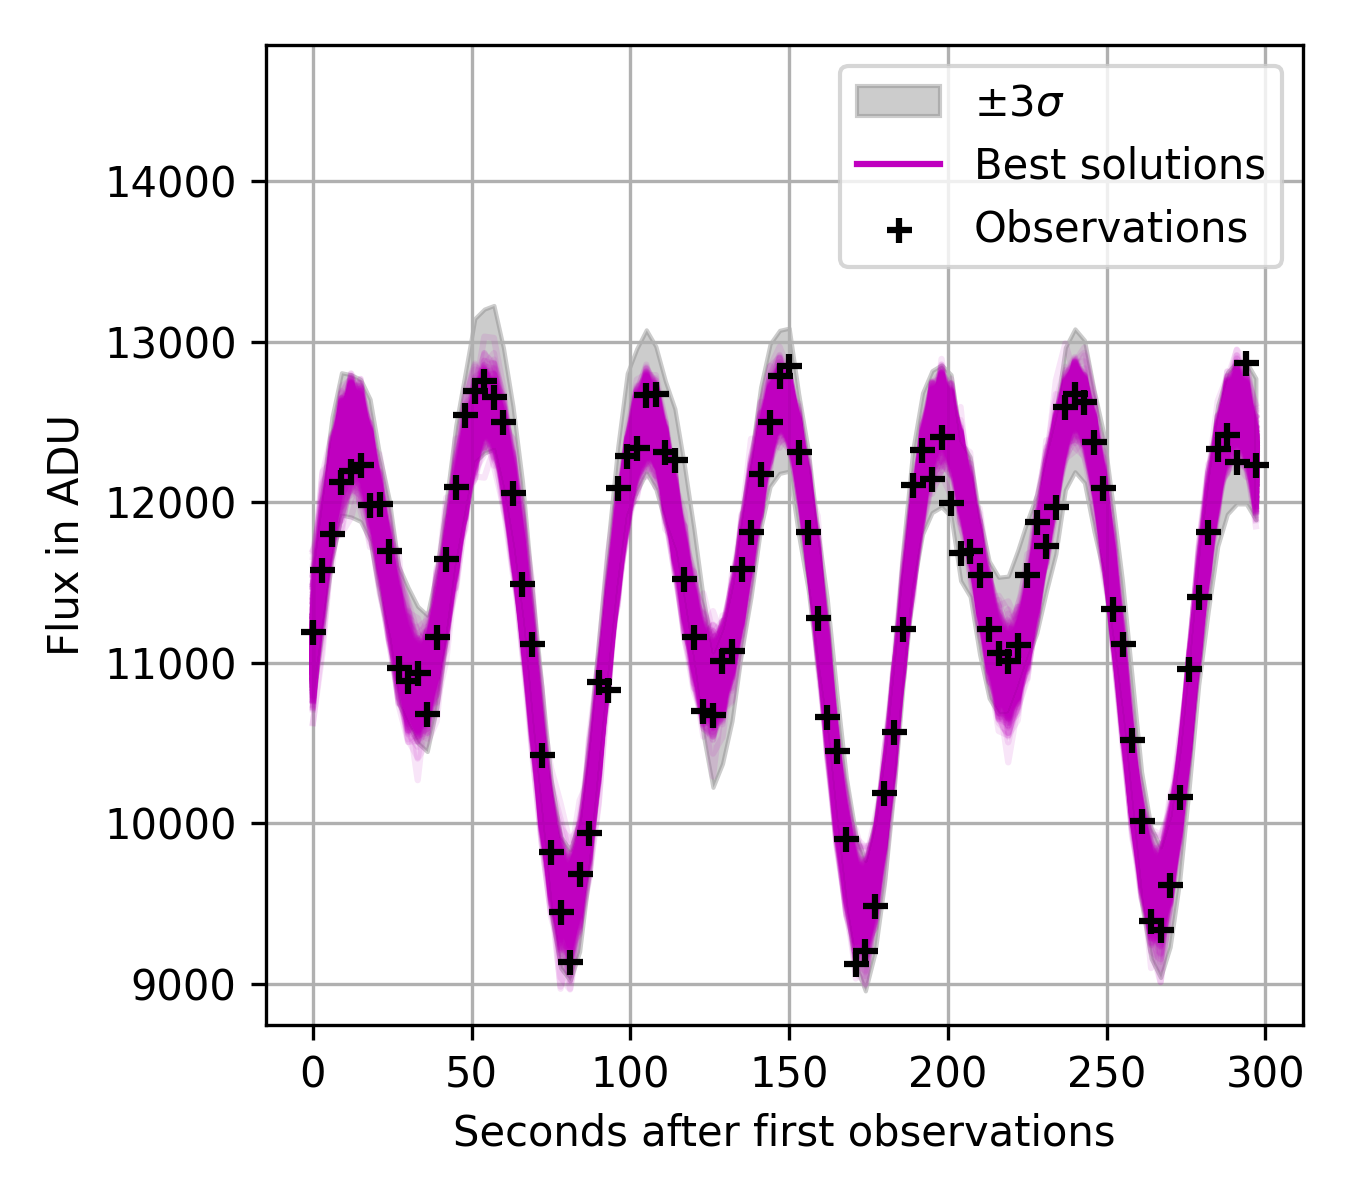
\includegraphics[width=\figmed]{converged_solutions_1_Rocket Body.png}
  \caption{Candidate solution light curves found through BFGS optimization.}
  \label{fig:conv_lcs_synth}
\end{figure}

Figures \ref{fig:sigma_sols1} and \ref{fig:omega_sols1} display the candidate MRP and angular velocity vectors of the best solutions determined via the procedure in Section \ref{sec:candidate_sols}. We notice that for both the initial orientation in Figure \ref{fig:sigma_sols1} and angular velocity in Figure \ref{fig:omega_sols1}, the ground truth, plotted in red, lies squarely on a candidate solution surface. In angular velocity space, shown in Figure \ref{fig:omega_sols1}, most solutions fall onto the surface of two open-ended cylinders -- one with half the radius of the larger cylinder containing the truth. Similarly in orientation space, shown in Figure \ref{fig:sigma_sols1}, the solutions fall on two distinct manifolds -- likely resulting from a reflection of the object's body frame about the bisector between the Sun and observer vectors \cite{marto2024, burton2024journal}. One of these orientation-space surfaces contains the ground truth. These additional families of solutions highlight the reality that a wide variety of attitude profiles may produce nearly identical observations.

\begin{figure}[H]
  \centering
  \begin{subfigure}[t]{0.23\textwidth}
    \centering
    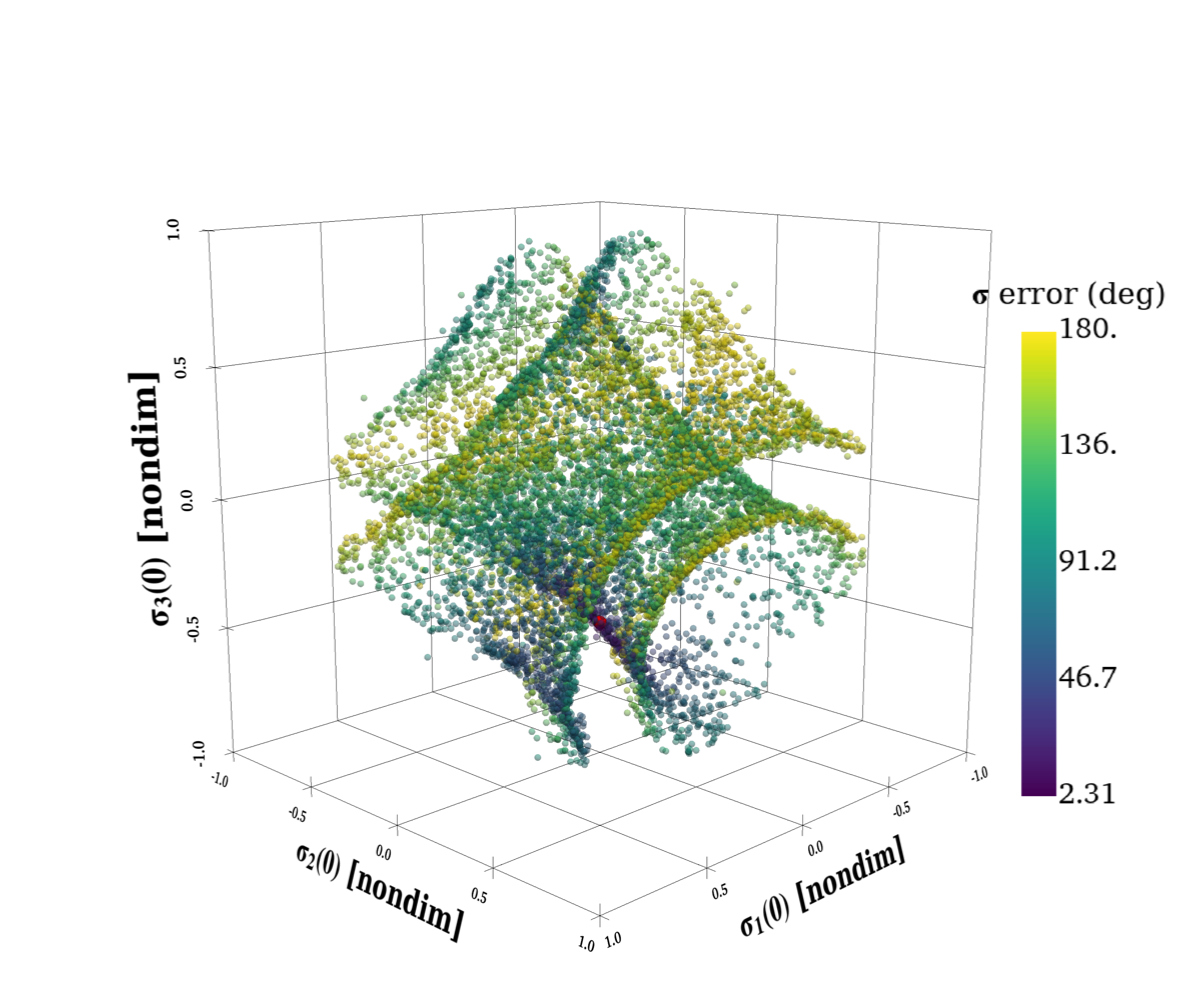
\includegraphics[width=\textwidth]{sigma_solsRocket Body.png}
    \caption{Uniform prior}
    \label{fig:sigma_sols1a}
  \end{subfigure}
  \hfill
  \begin{subfigure}[t]{0.23\textwidth}
    \centering
    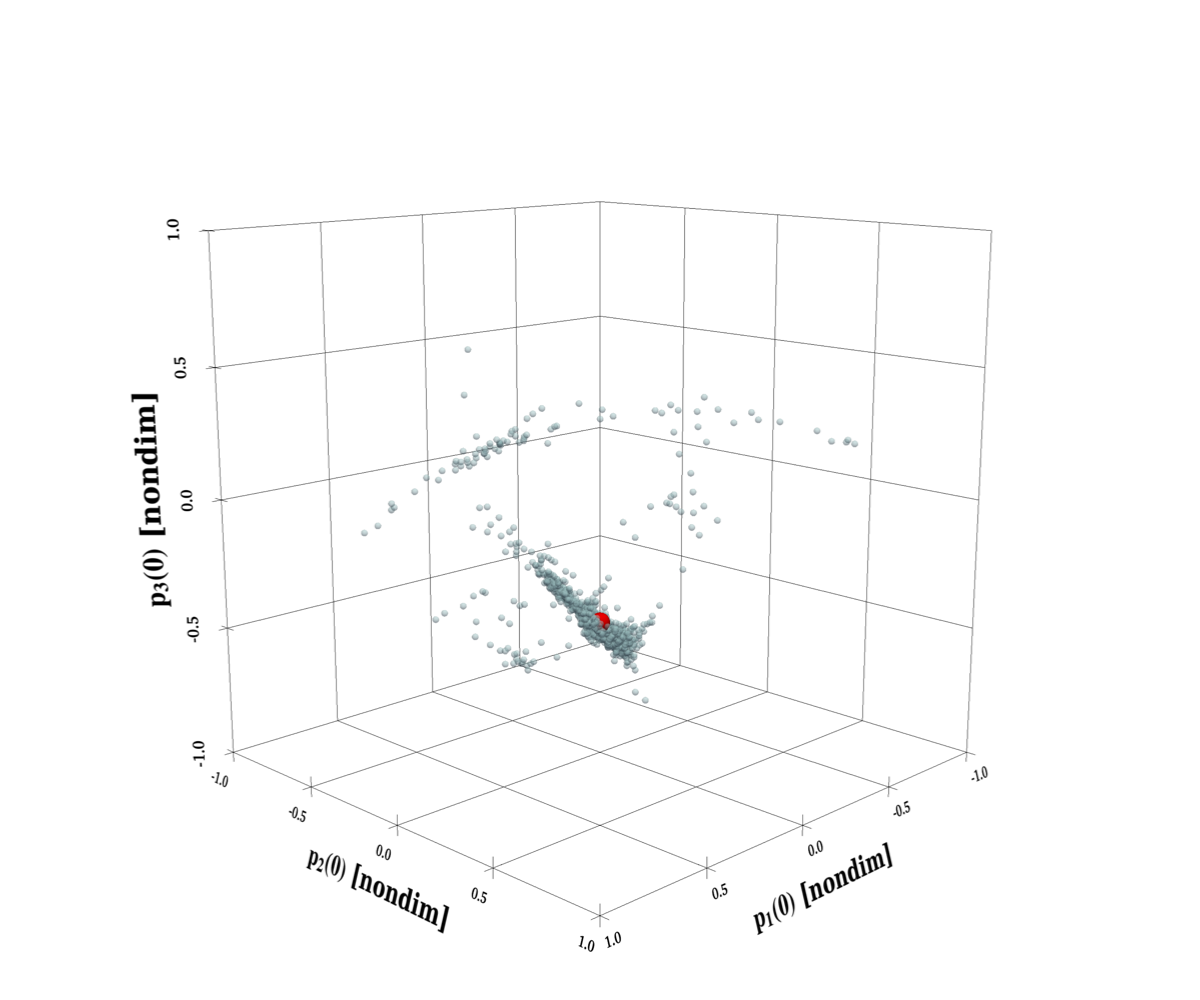
\includegraphics[width=\textwidth]{sigma_solsRocket Body Prior.png}
    \caption{Informative prior}
    \label{fig:sigma_sols1b}
  \end{subfigure}

  \caption{Candidate solution initial orientation MRP vectors, ground truth highlighted in red.}
  \label{fig:sigma_sols1}
\end{figure}

\begin{figure}[H]
  \centering
  \begin{subfigure}[t]{0.23\textwidth}
    \centering
    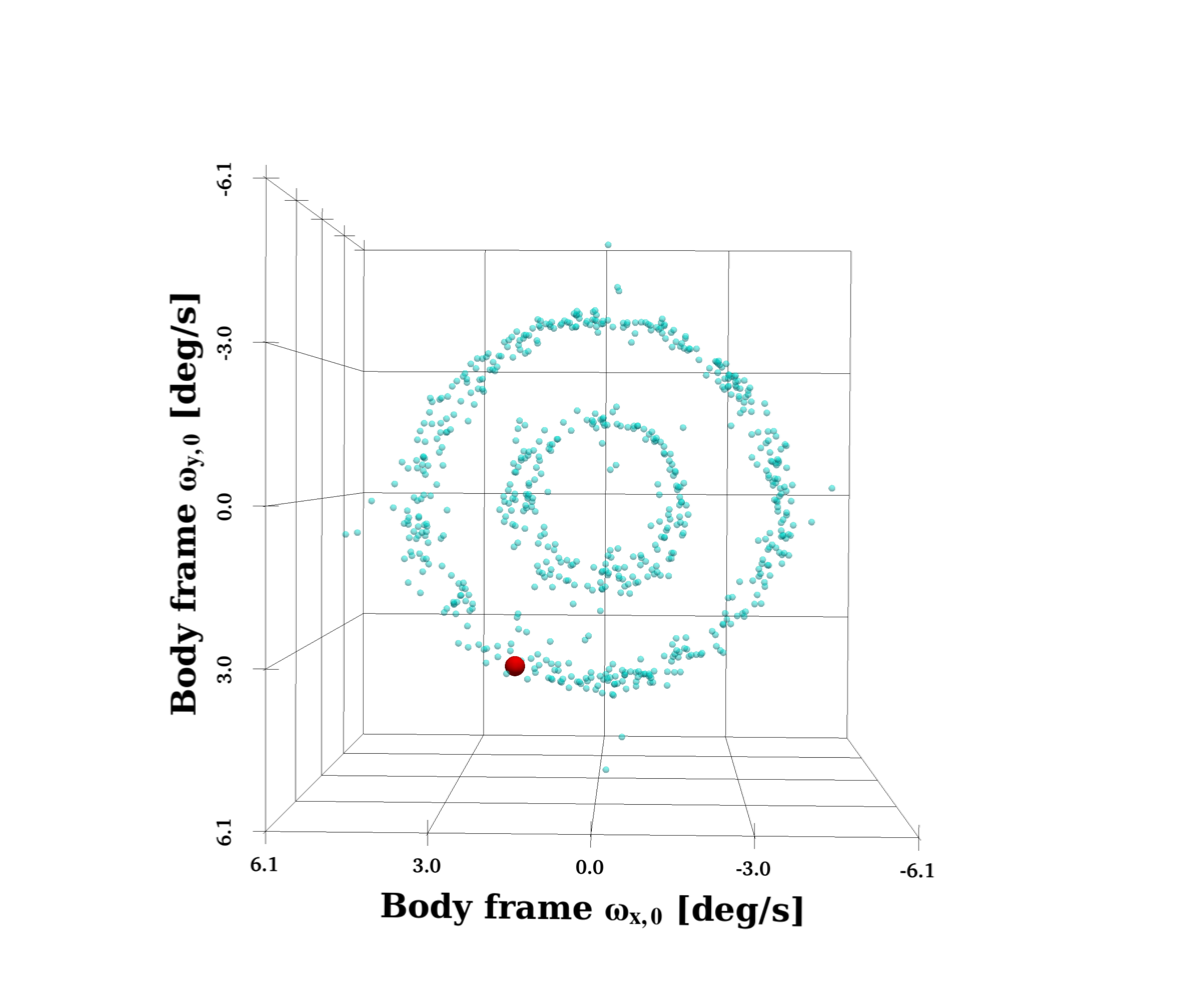
\includegraphics[width=\textwidth]{omega_sols_Rocket Body.png}
    \caption{Uniform prior}
    \label{fig:omega_sols1a}
  \end{subfigure}
  \hfill
  \begin{subfigure}[t]{0.23\textwidth}
    \centering
    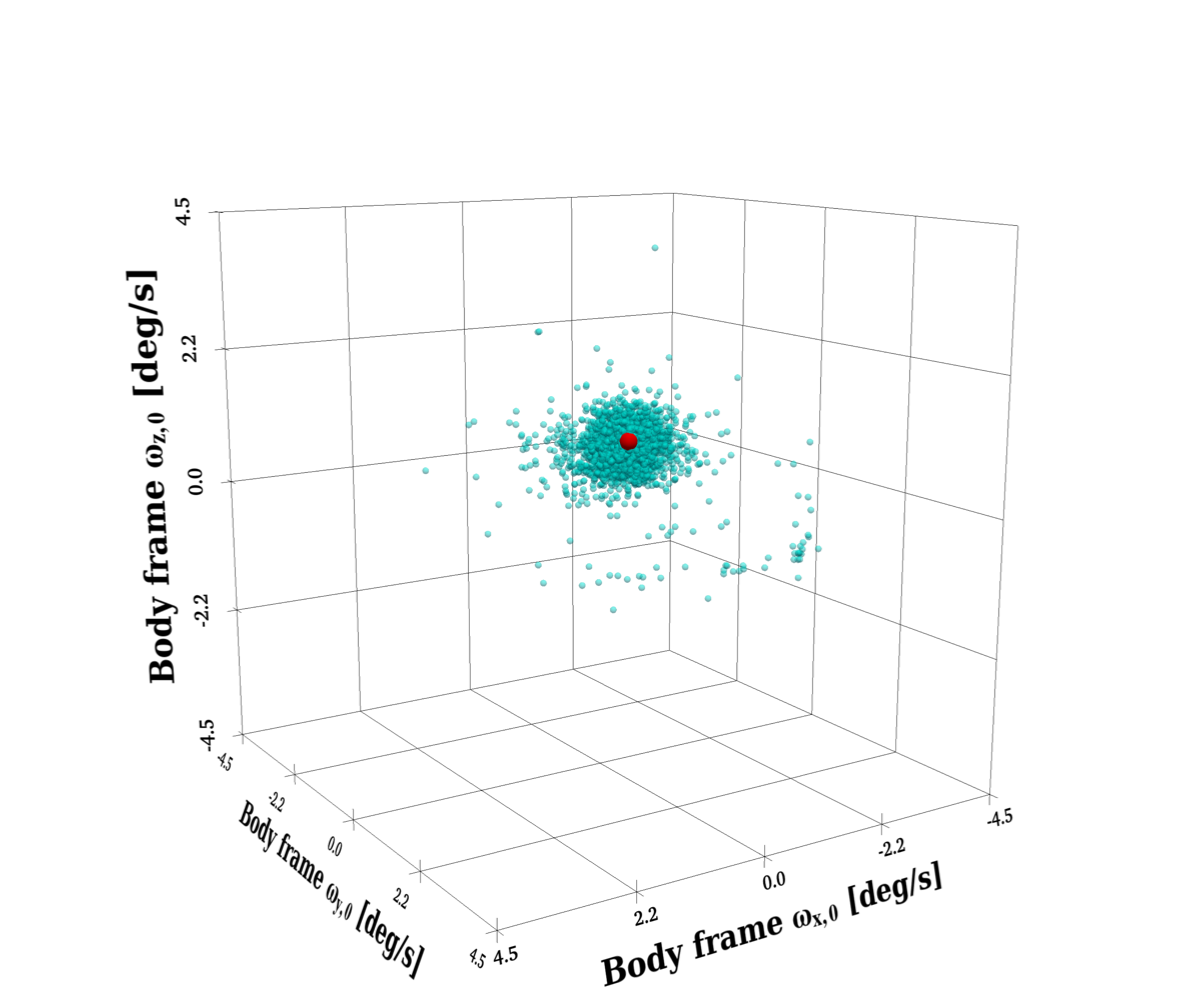
\includegraphics[width=\textwidth]{omega_sols_Rocket Body Prior.png}
    \caption{Informative prior}
    \label{fig:omega_sols1b}
  \end{subfigure}

  \caption{Candidate solution initial body-frame angular velocity vectors, ground truth highlighted in red. TODO: change the perspective on the angular velocities}
  \label{fig:omega_sols1}
\end{figure}

\begin{figure}[H]
  \centering
  \begin{subfigure}[t]{0.23\textwidth}
    \centering
    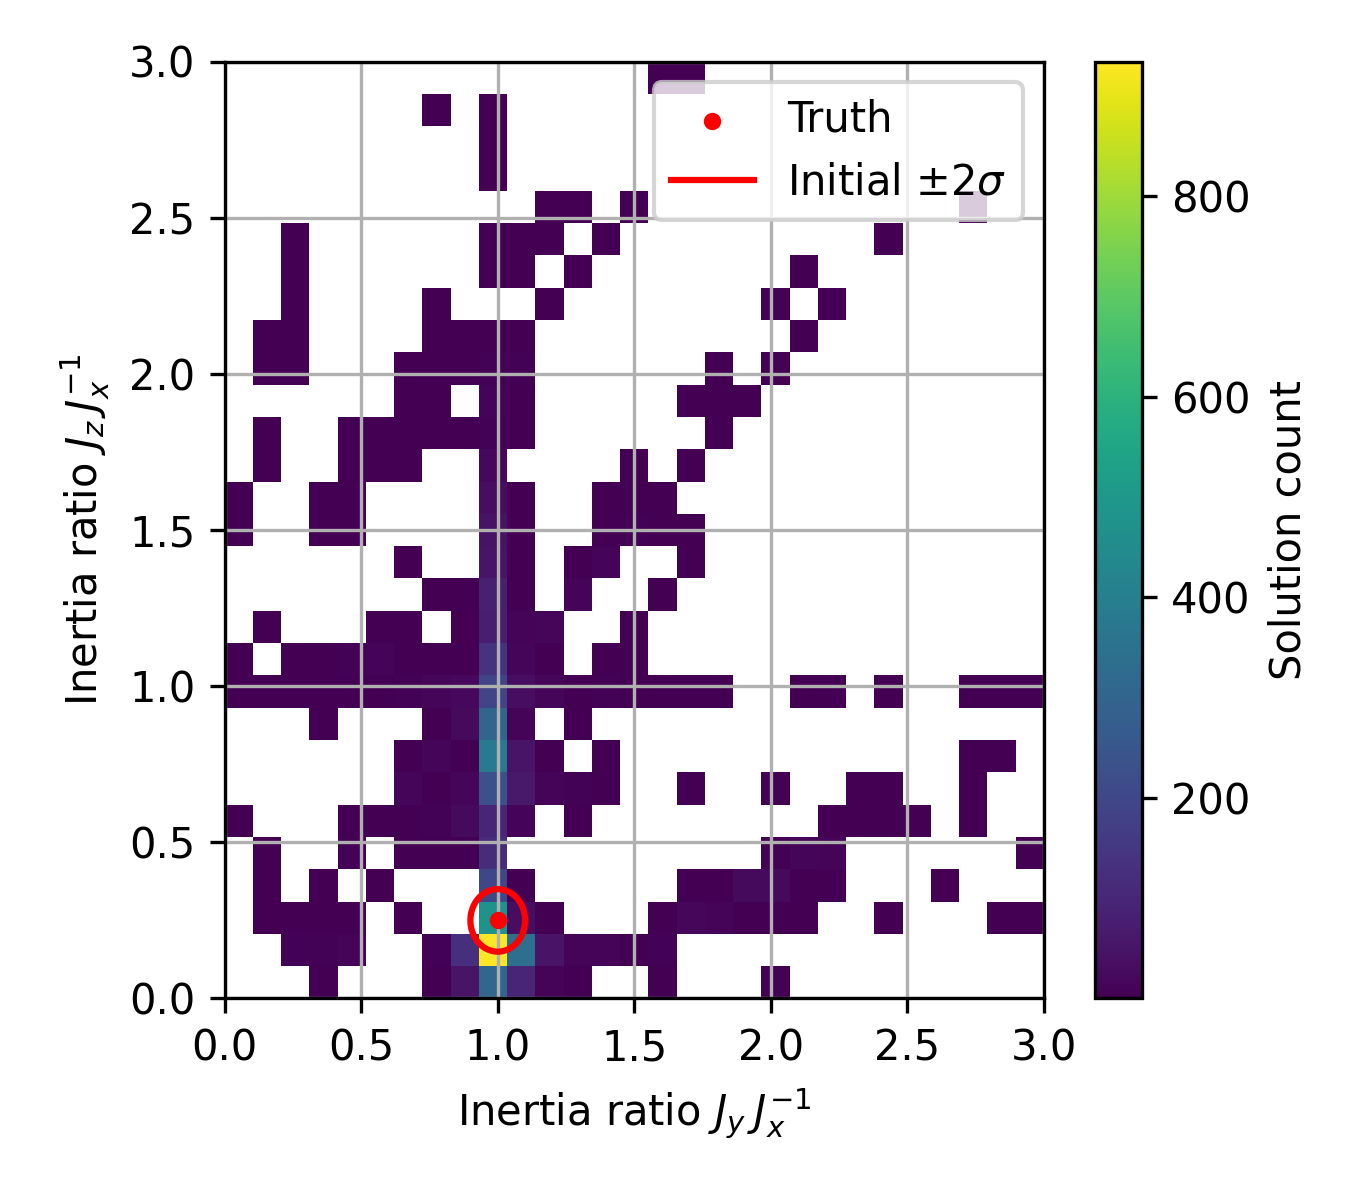
\includegraphics[width=\textwidth]{converged_solutions_2_Rocket Body.png}
    \caption{Uniform prior}
    \label{fig:i_sols1a}
  \end{subfigure}
  \hfill
  \begin{subfigure}[t]{0.23\textwidth}
    \centering
    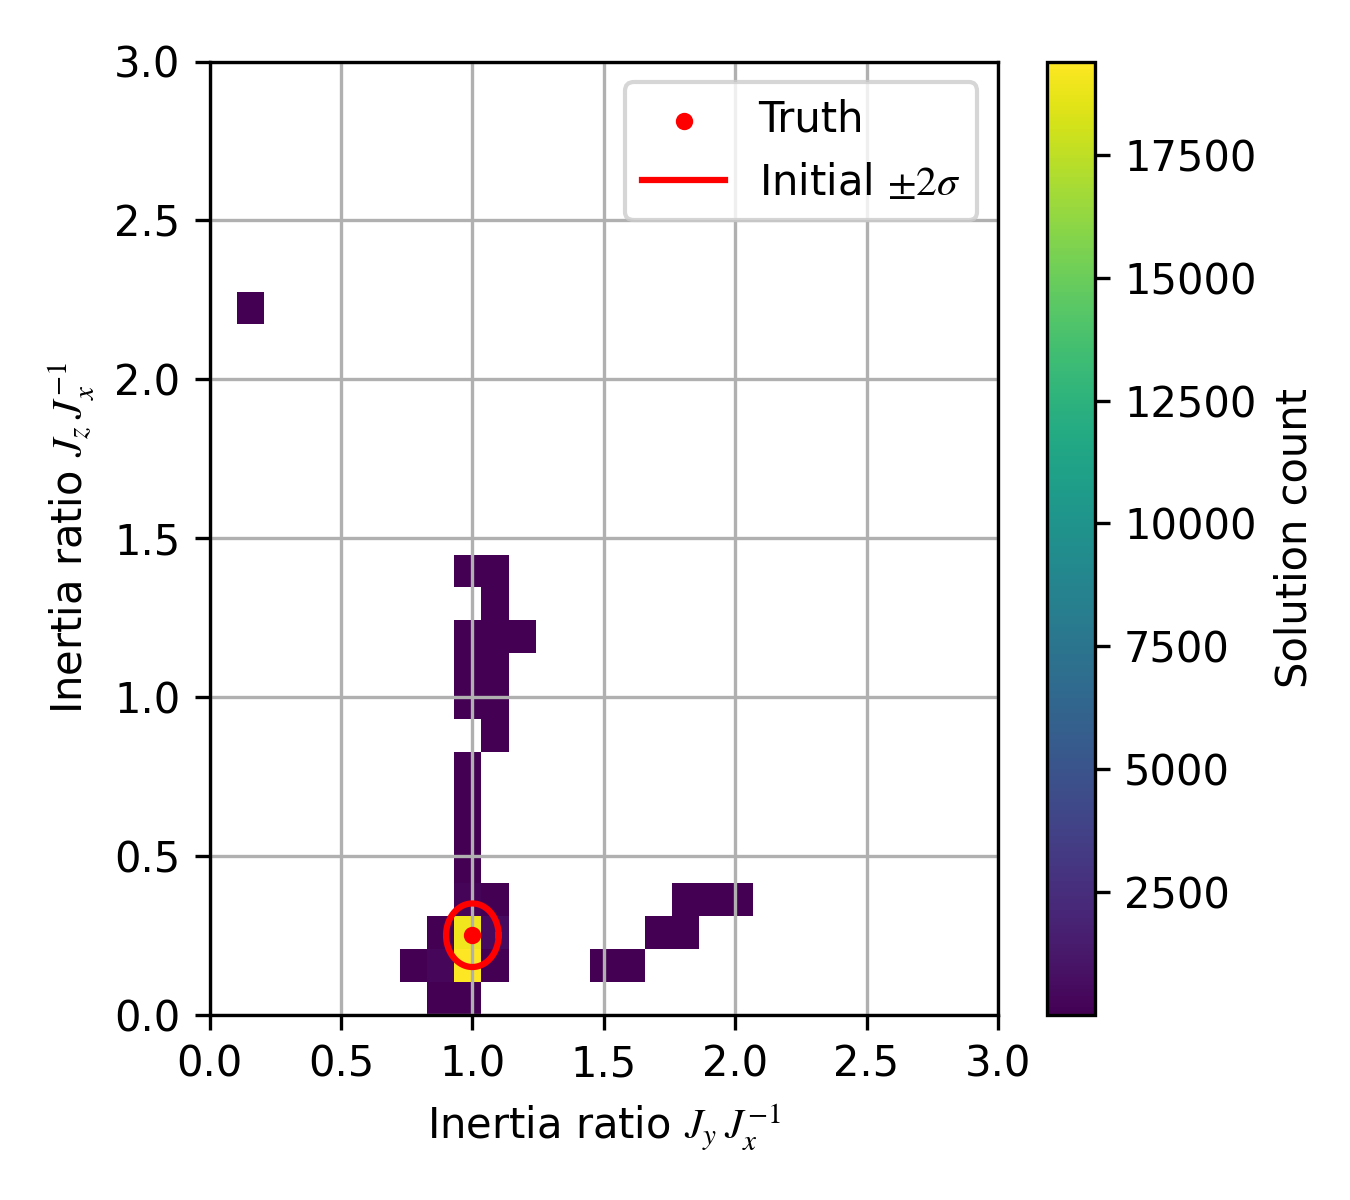
\includegraphics[width=\textwidth]{converged_solutions_2_Rocket Body Prior.png}
    \caption{Informative prior}
    \label{fig:i_sols1b}
  \end{subfigure}

  \caption{Candidate solution inertia ratios, ground truth highlighted in red.}
  \label{fig:i_sols1}
\end{figure}

\begin{figure}[H]
  \centering
  \begin{subfigure}[t]{0.23\textwidth}
    \centering
    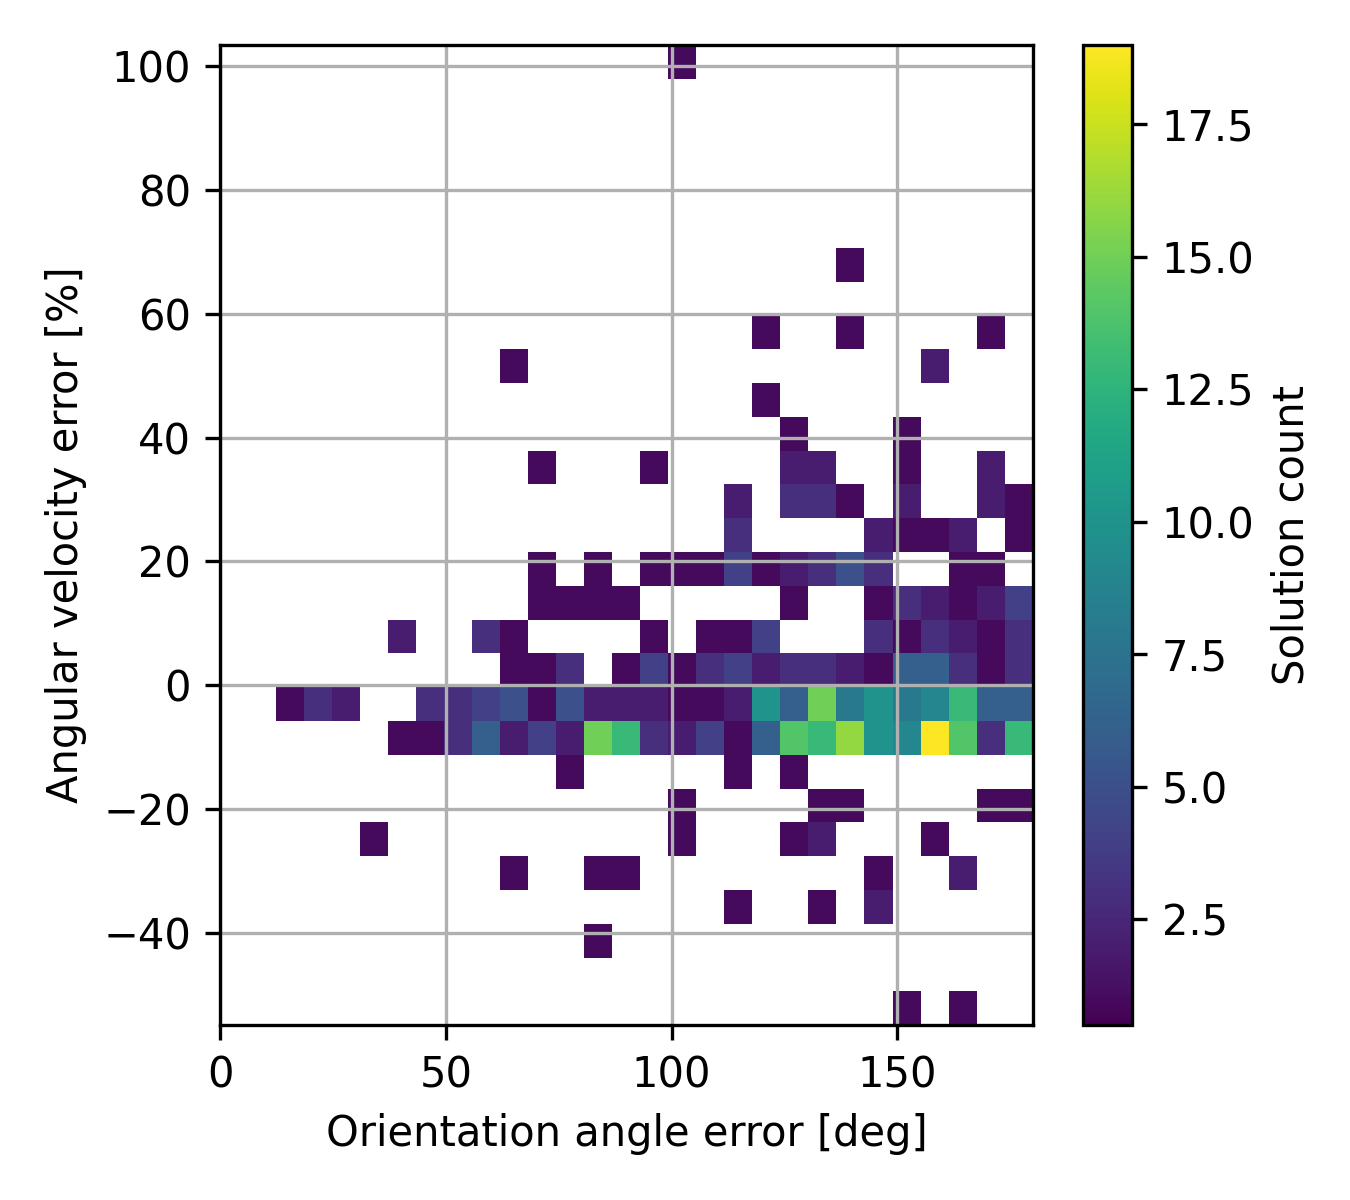
\includegraphics[width=\textwidth]{converged_solutions_3_Rocket Body.png}
    \caption{Uniform prior}
    \label{fig:w_vs_ang_error_sols1a}
  \end{subfigure}
  \hfill
  \begin{subfigure}[t]{0.23\textwidth}
    \centering
    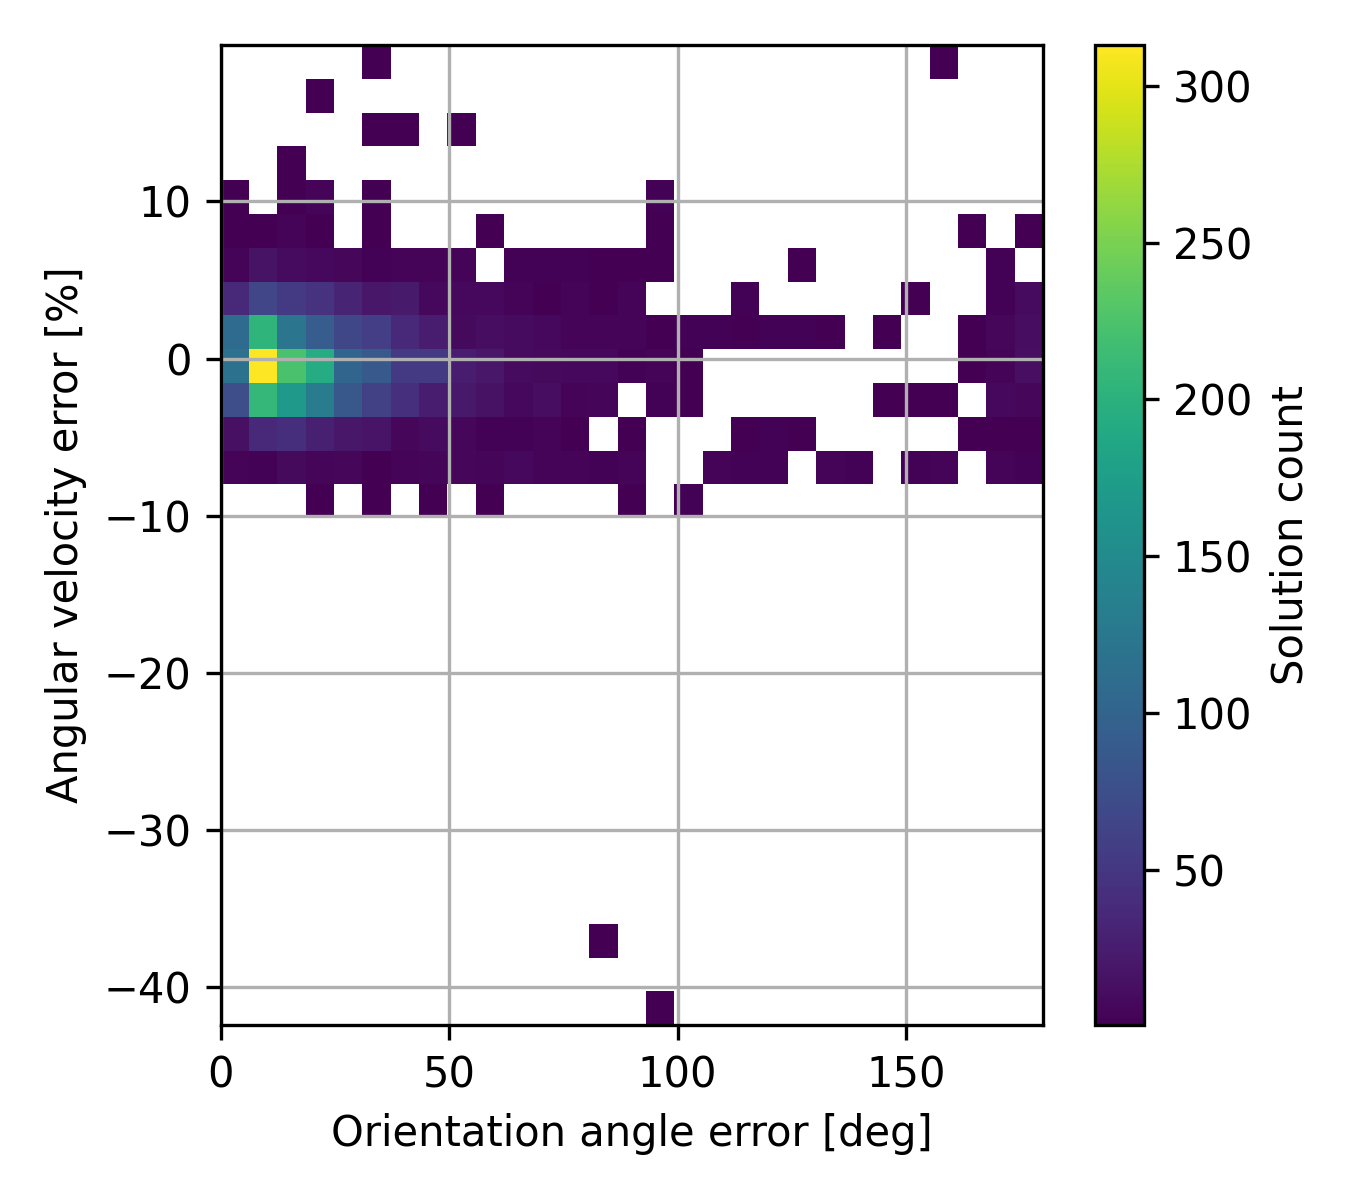
\includegraphics[width=\textwidth]{converged_solutions_3_Rocket Body Prior.png}
    \caption{Informative prior}
    \label{fig:w_vs_ang_error_sols1b}
  \end{subfigure}

  \caption{Candidate solution angular orientation error and angular velocity magnitudes compared to the truth}
  \label{fig:w_vs_ang_error_sols1}
\end{figure}

% While the state vectors of the candidate solutions do not uniquely indicate the ground truth, the object's precession rate is estimated

% \begin{figure}[H]
%   \centering
%   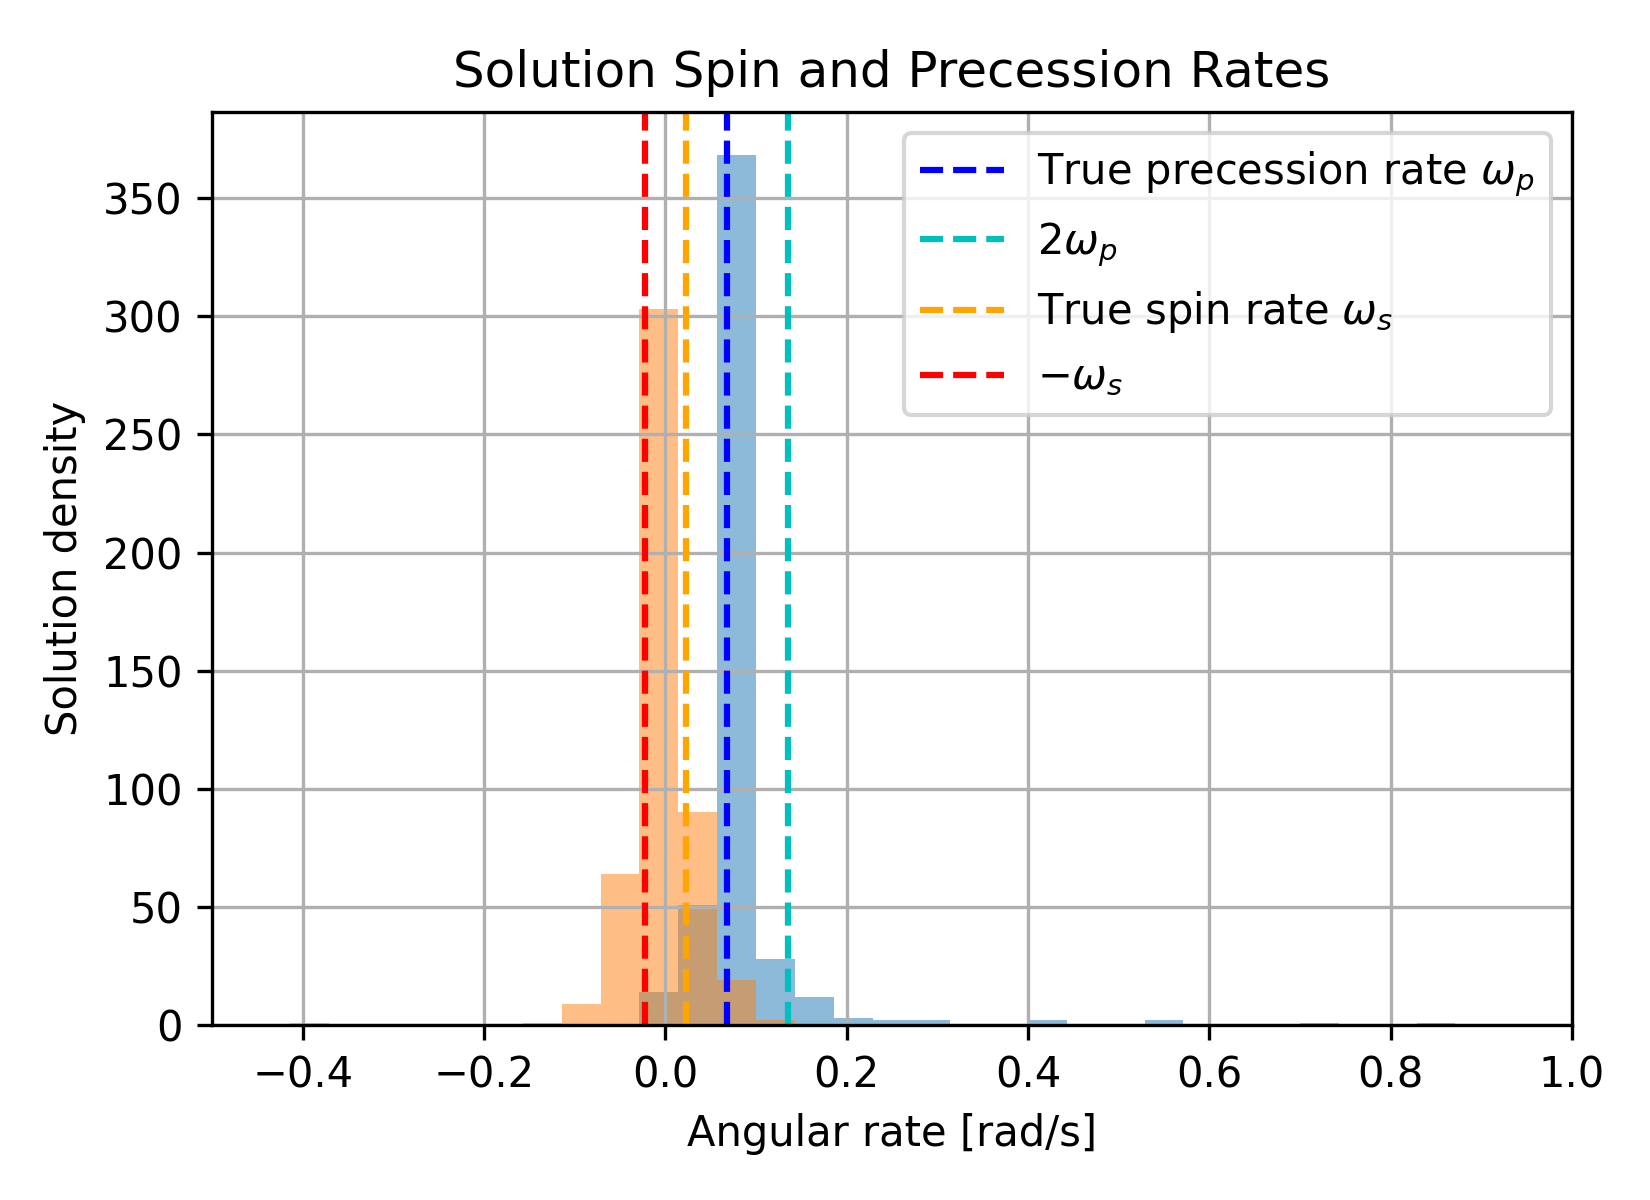
\includegraphics[width=\figsmall]{spin_proc_Rocket Body.png}
%   \caption{Converged solution body frame spin and precession rates.}
%   \label{fig:spin_proc1}
% \end{figure}

% The inversion 

\section{Attitude Inversion Results for Real Data}

% The two objects selected for study in this work are a Delta I upper stage and the ECHOSTAR 2 satellite.

\subsection{Delta I Upper Stage}

The Delta I upper stage (COSPAR ID 1984-115C) is a Star-37E \cite{delta3914_astronautix} solid fuel apogee kick motor, displayed in Figure \ref{fig:star37e}. It is $d=0.93$ meters in diameter and is approximately $h=1.7$ meters in length \cite{star37e_astronautix, star37_gunter}.

\begin{figure}[H]
  \centering
  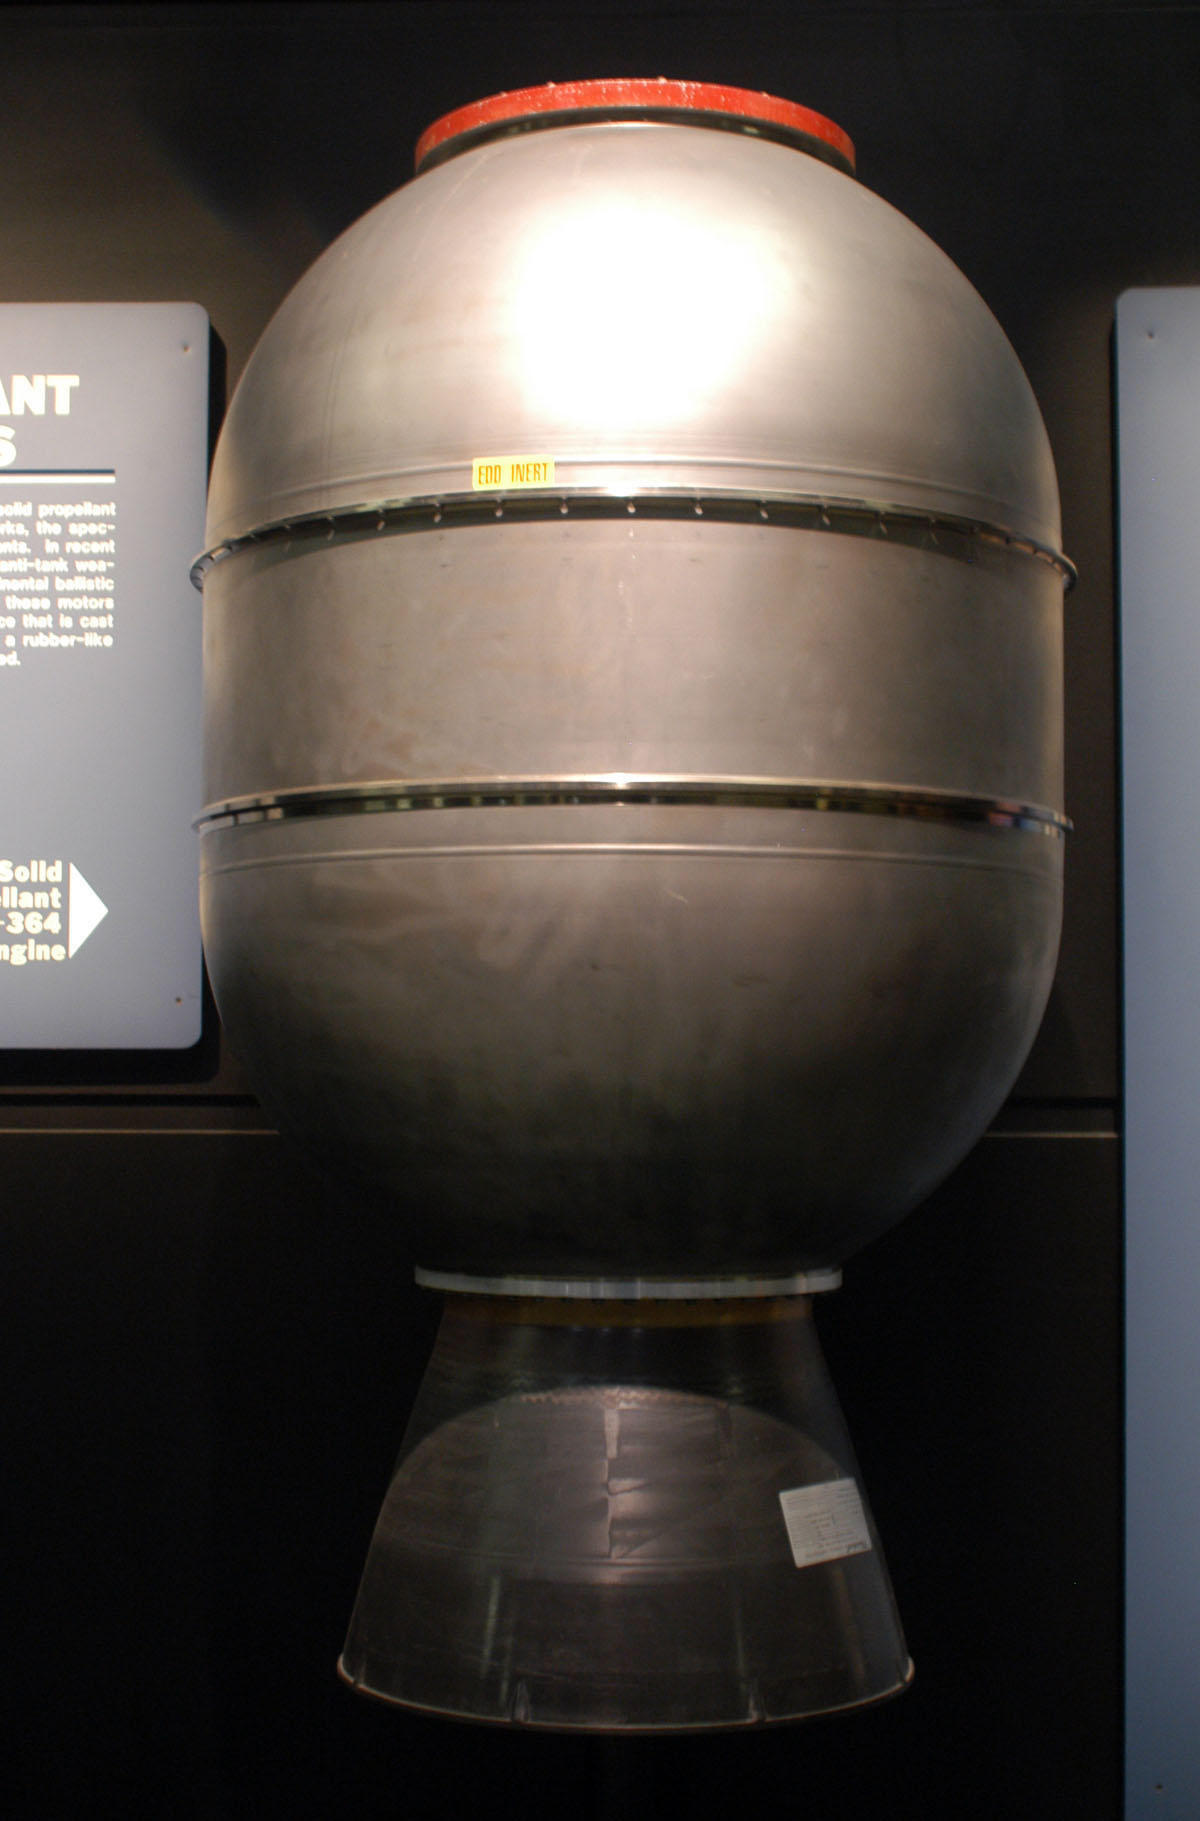
\includegraphics[width=\figsmall]{star37e.JPG}
  \caption{Star-37E upper stage \cite{star37_af}.}
  \label{fig:star37e}
\end{figure}

\begin{figure}[H]
  \centering
  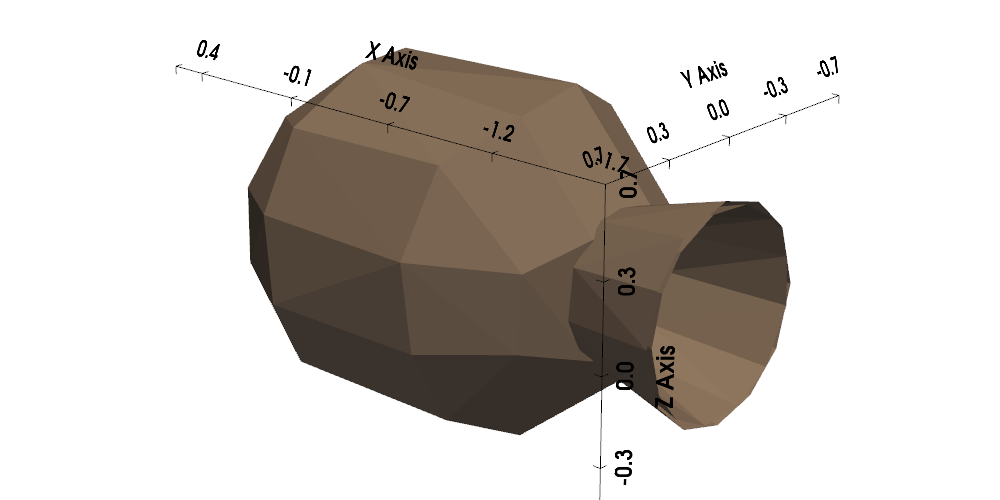
\includegraphics[width=\figbig]{sphx_glr_plot_models_002.png}
  \caption{Simplified Star-37E model used for inversion.}
  \label{fig:star37e_simple}
\end{figure}

We compute the inertia tensor of the Star-37E by approximating its geometry as a hollow cylinder of the same aspect ratio such that \cite{serway2019}:

\begin{align}
 J_a &= \frac{1}{2} m \left(r_o^2+r_i^2\right) \\
 J_t &= \frac{1}{12} m \left(3 \left(r_o^2+r_i^2\right) + h^2\right) \\
 J_\text{R/B} &= \text{diag} \left(J_a, J_t, J_t\right).
\end{align}

Here, we choose the inner radius to be $r_i=0.45d$, the outer radius to be $r_o=0.5d$, and $m=1$ kilogram -- dividing each moment of inertia by a constant does not change the dynamics -- yielding $J_a = 15.3 \: [kg \cdot m^2]$ and $J_t = 27.9 \: [kg \cdot m^2]$. Table \ref{tb:case2_in} summarizes the light curve observations that result in the extracted measurements displayed in Figure \ref{fig:rb_lc_obs}.

\begin{table}[H]
  \centering
  \caption{Delta I rocket body observation characteristics}
  \vspace*{6pt}
  \begin{tabular}{|l|l|}
  \hline
  \textbf{Variable} & \textbf{Value} \\ \hline
 Target COSPAR ID & 1984-115C \\ \hline
 First obs.\ (UTC) & Mar 2, 2025 01:53:30.251 \\ \hline
 Light curve duration & $7.5$ minutes \\ \hline
 Observations & $100$ ($92$ extracted) \\ \hline
 Obs.\ frequency & $0.222$ Hz \\ \hline
 Integration time & $3$ seconds \\ \hline
  \end{tabular}
  \label{tb:case2_in}
\end{table}

\begin{figure}[H]
  \centering
  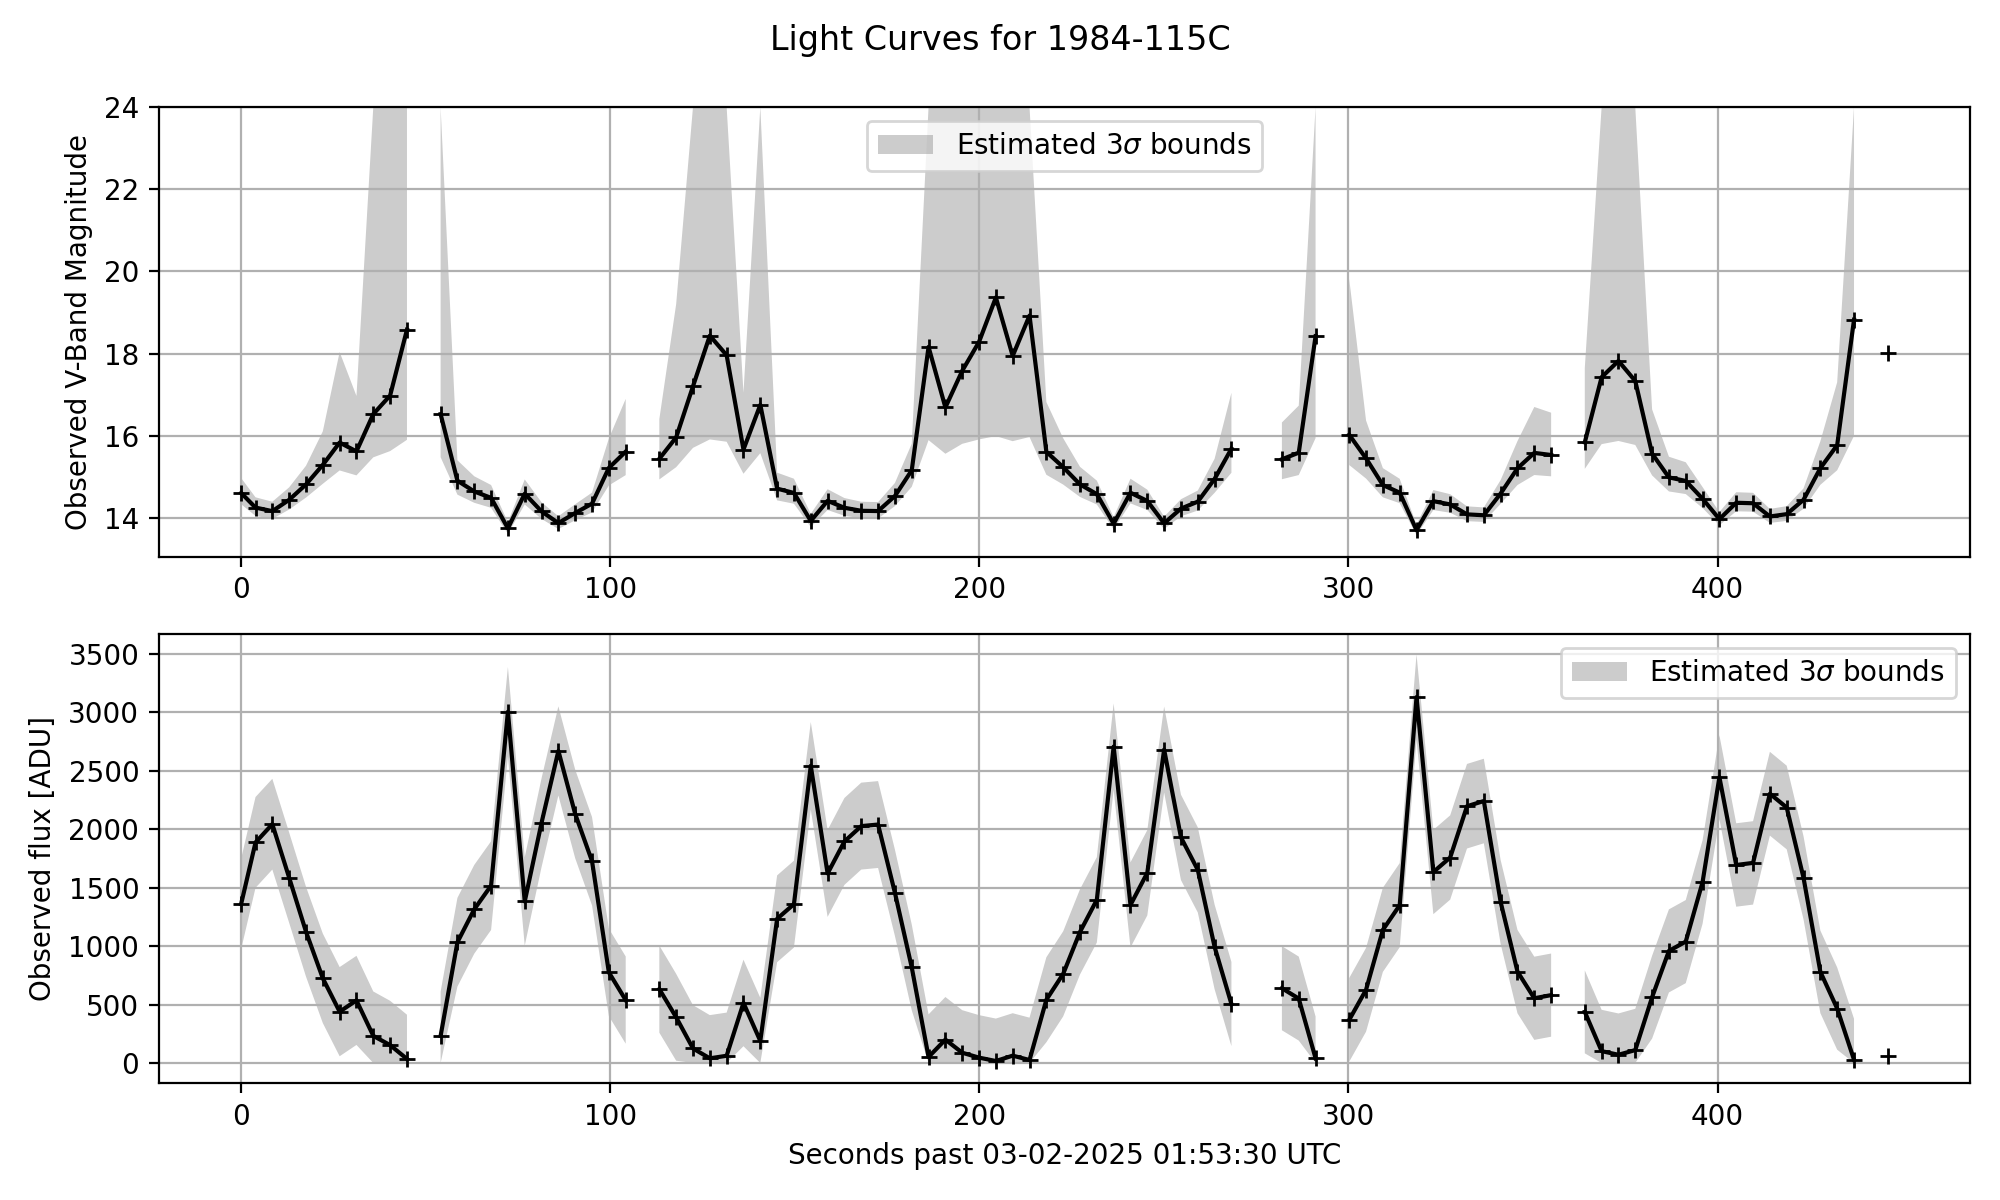
\includegraphics[width=\figbig]{sphx_glr_plot_lcs_001_2_00x.png}
  \caption{Selected light curve for the Delta I (Star-37E) rocket body, observed by the Purdue Optical Ground Station}
  \label{fig:rb_lc_obs}
\end{figure}

This light curve shows clear periodicity, but has a high measurement standard deviation and a relatively low sampling rate due to the object's low brightness and the sensor readout time. Inversion was performed using $10^4$ initial guesses with the material and angular velocity assumptions listed in Table \ref{tb:case2_ass}. The candidate solution results are presented in terms of their mean light curves in Figure \ref{fig:case2_s}, orientation MRPs and angular velocities in Figure \ref{fig:case2_pw}, and inertia ratios in Figure \ref{fig:case2_i}.

\begin{table}[H]
  \centering
  \caption{Delta I rocket body inversion assumptions}
  \vspace*{6pt}
  \begin{tabular}{|l|l|}
  \hline
  \textbf{Variable} & \textbf{Value} \\ \hline
 Uniform BRDF & $C_d=0.2$, $C_s=0.8$, $n=30$ \\ \hline
 $\norm{\vctr{\omega}}_\text{max}$ & $8.31$ $\text{deg} / \text{s}^{-1}$ \\ \hline
 $\ell$ & $1/100$ \\ \hline
\end{tabular}
  \label{tb:case2_ass}
\end{table}

\begin{figure*}[t]
  \centering
  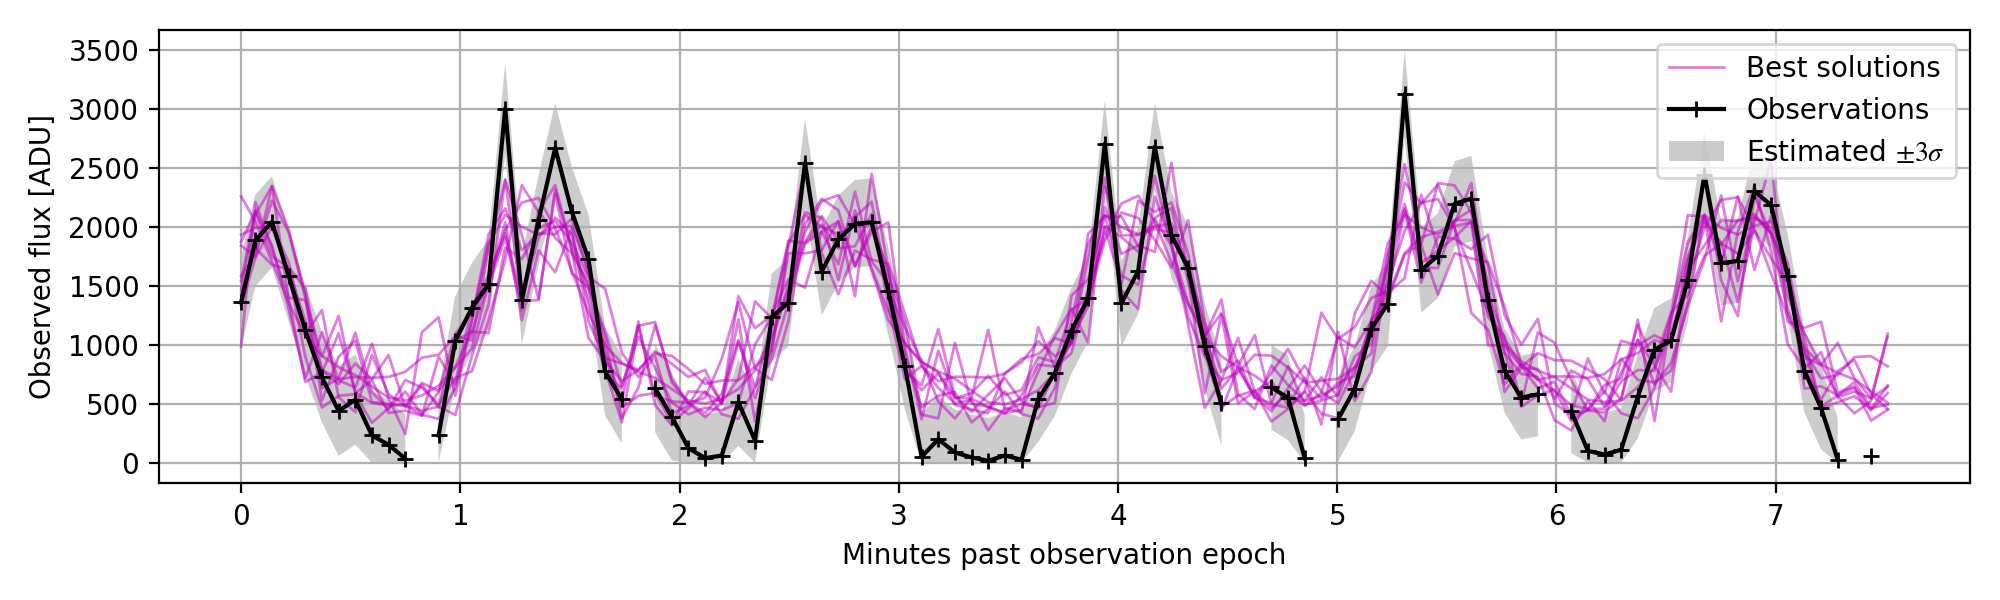
\includegraphics[width=0.8\textwidth]{sphx_glr_results_002_2_00x.png}
  \caption{Candidate solution light curves compared to the real measurements in ADU for the Delta I (Star-37E) rocket body.}
  \label{fig:case2_s}
\end{figure*}

% \begin{figure}[H]
%   \centering
%   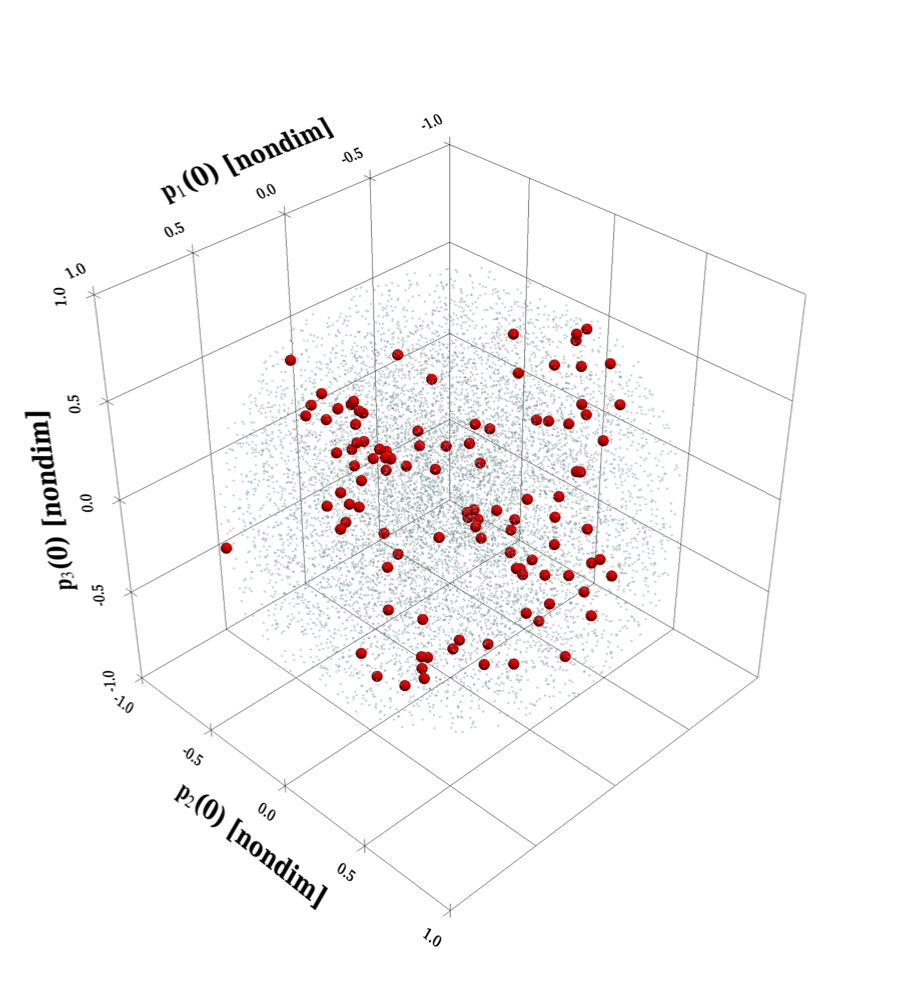
\includegraphics[width=\figmed]{sphx_glr_results_006.png}
%   \caption{}
%   \label{fig:case2_p}
% \end{figure}

\begin{figure}[H]
  \centering
  \begin{subfigure}[t]{0.23\textwidth}
    \centering
    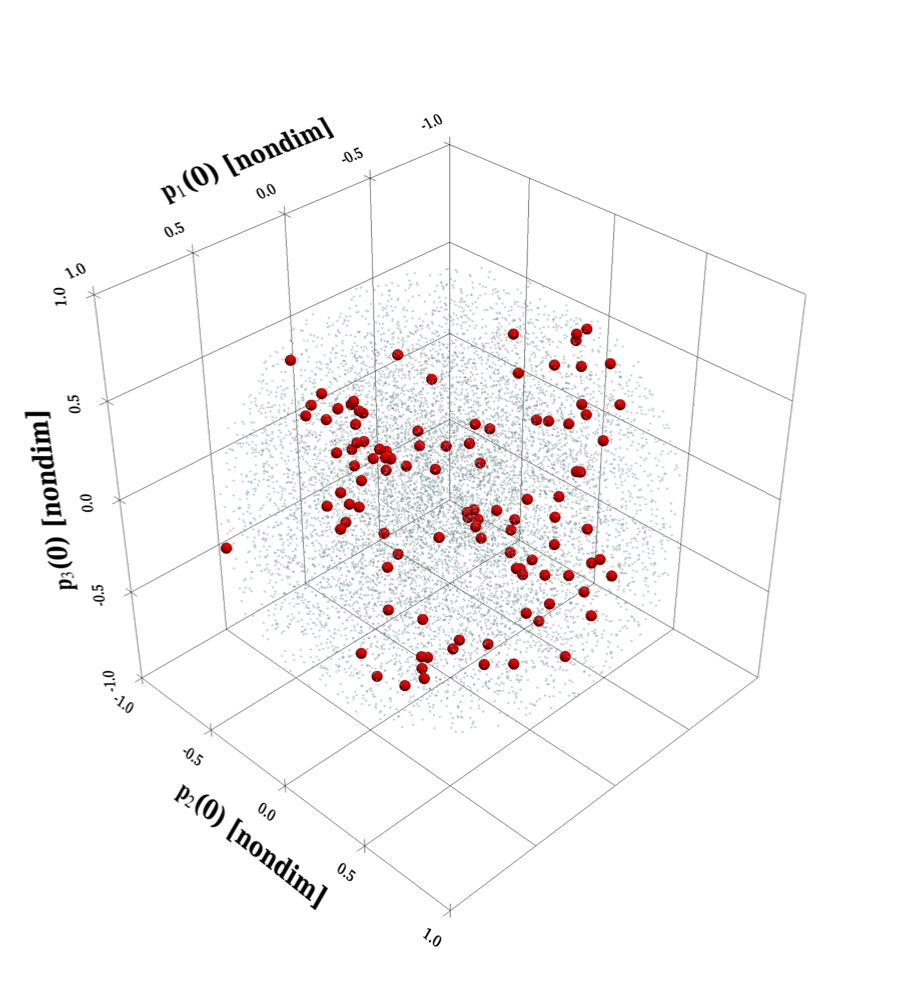
\includegraphics[width=\textwidth]{sphx_glr_results_006.png}
    \caption{MRP}
    \label{fig:case2_pwa}
  \end{subfigure}
  \hfill
  \begin{subfigure}[t]{0.23\textwidth}
    \centering
    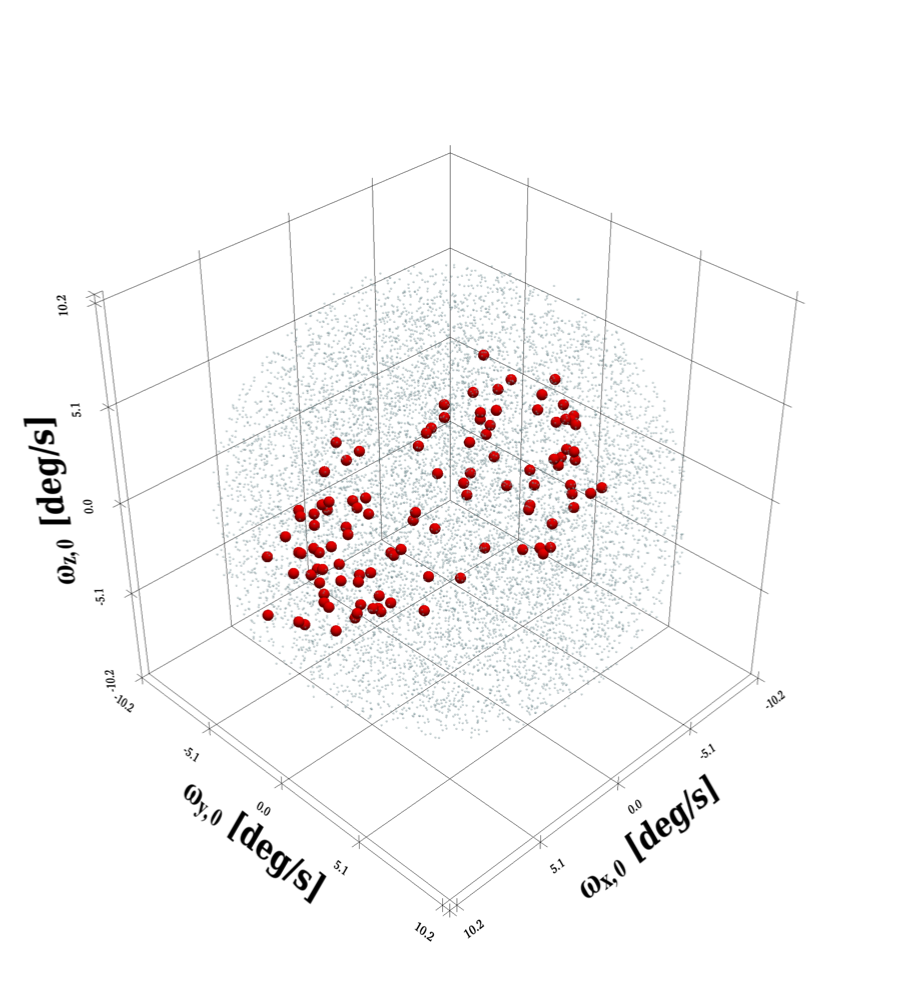
\includegraphics[width=\textwidth]{sphx_glr_results_005.png}
    \caption{Angular velocity}
    \label{fig:case2_pwb}
  \end{subfigure}

  \caption{Candidate solution orientation MRPs and angular velocity vectors for the Delta I (Star-37E) rocket body}
  \label{fig:case2_pw}
\end{figure}

% \begin{figure}[H]
%   \centering
%   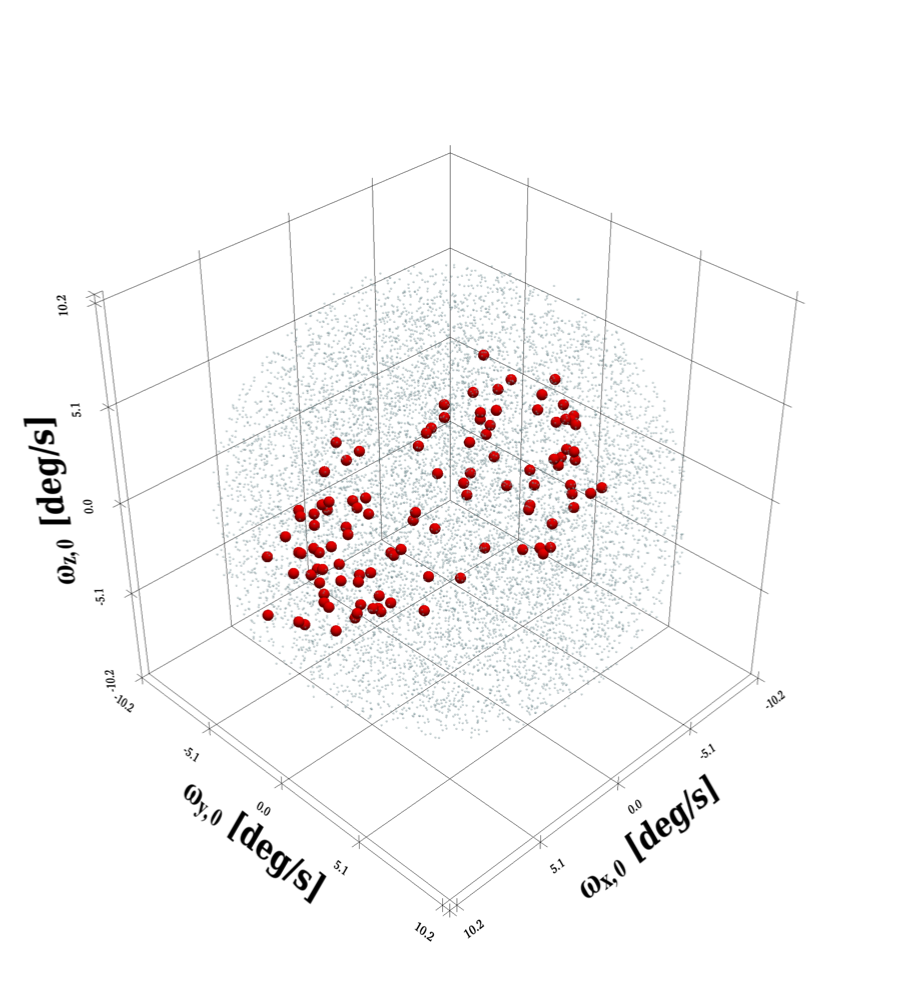
\includegraphics[width=\figmed]{sphx_glr_results_005.png}
%   \caption{Candidate solution angular velocities for the Delta I (Star-37E) rocket body}
%   \label{fig:case2_w}
% \end{figure}

\begin{figure}[H]
  \centering
  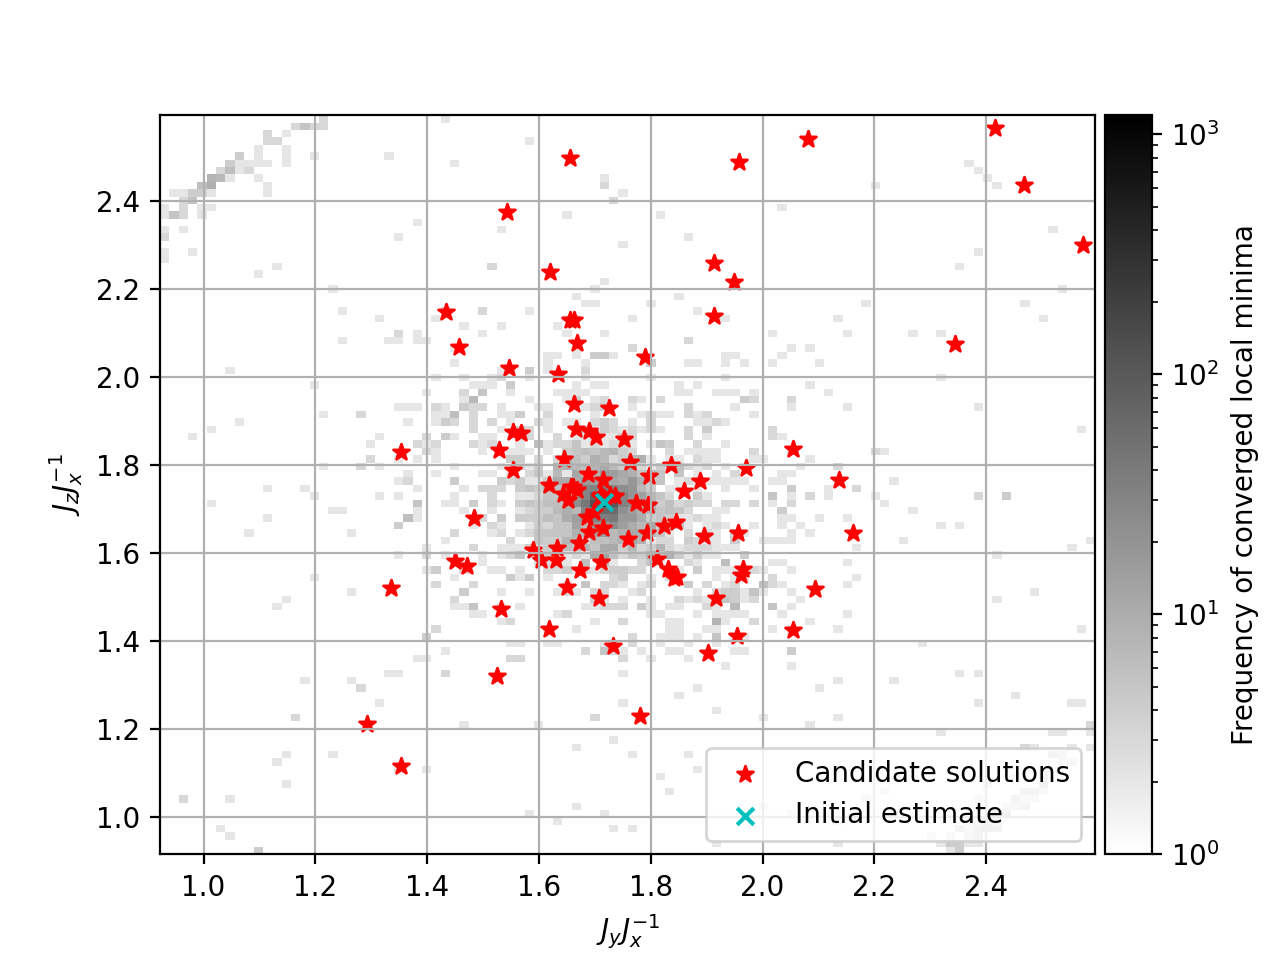
\includegraphics[width=\figmed]{sphx_glr_results_001_2_00x.png}
  \caption{Candidate solution inertia ratio distribution for the Delta I (Star-37E) rocket body}
  \label{fig:case2_i}
\end{figure}

The candidate solutions identified by the inversion process produce light curves which adequately approximate the measurements, although they do not reach the lowest observed values. This indicates that the true material is more dominated by specular reflections than our assumed coefficients. The candidates show some rough clustering in both orientation and angular velocity space, although they vary significantly in angular velocity magnitude. The inertia tensor solutions display similar variability, although the solutions are spread relatively uniformly from the initial guess, possibly indicating that it was reasonably unbiased. Taken together, these results indicate that the object could be spinning in a number of attitude profiles, and that more information is needed about its true mass distribution and reflectivity to further refine the solution set.

\subsection{ECHOSTAR II}

ECHOSTAR II (COSPAR ID 1996-055A) was a communications satellite on the AS-7000 bus \cite{as7000_astronautix}, shown in Figure \ref{fig:echostar1}. It has an approximate total wingspan of $s = 23.9$ meters, individual solar panel length of $l_p=8.5$ meters, panel width of $w_p=3.1$ meters, and a mass per panel of $m_p = 60$ kilograms \cite{earl2015}. The spacecraft bus is approximately cubic with a side length $w_b=2.3$ meters and a mass of $m_b = 1900$ kilograms \cite{earl2015}.

\begin{figure}[H]
  \centering
  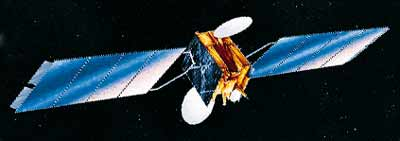
\includegraphics[width=\figbig]{EchoStar-1_image.jpg}
  \caption{ECHOSTAR II artist's rendition \cite{as7000_astronautix}.}
  \label{fig:echostar1}
\end{figure}

\begin{figure}[H]
  \centering
  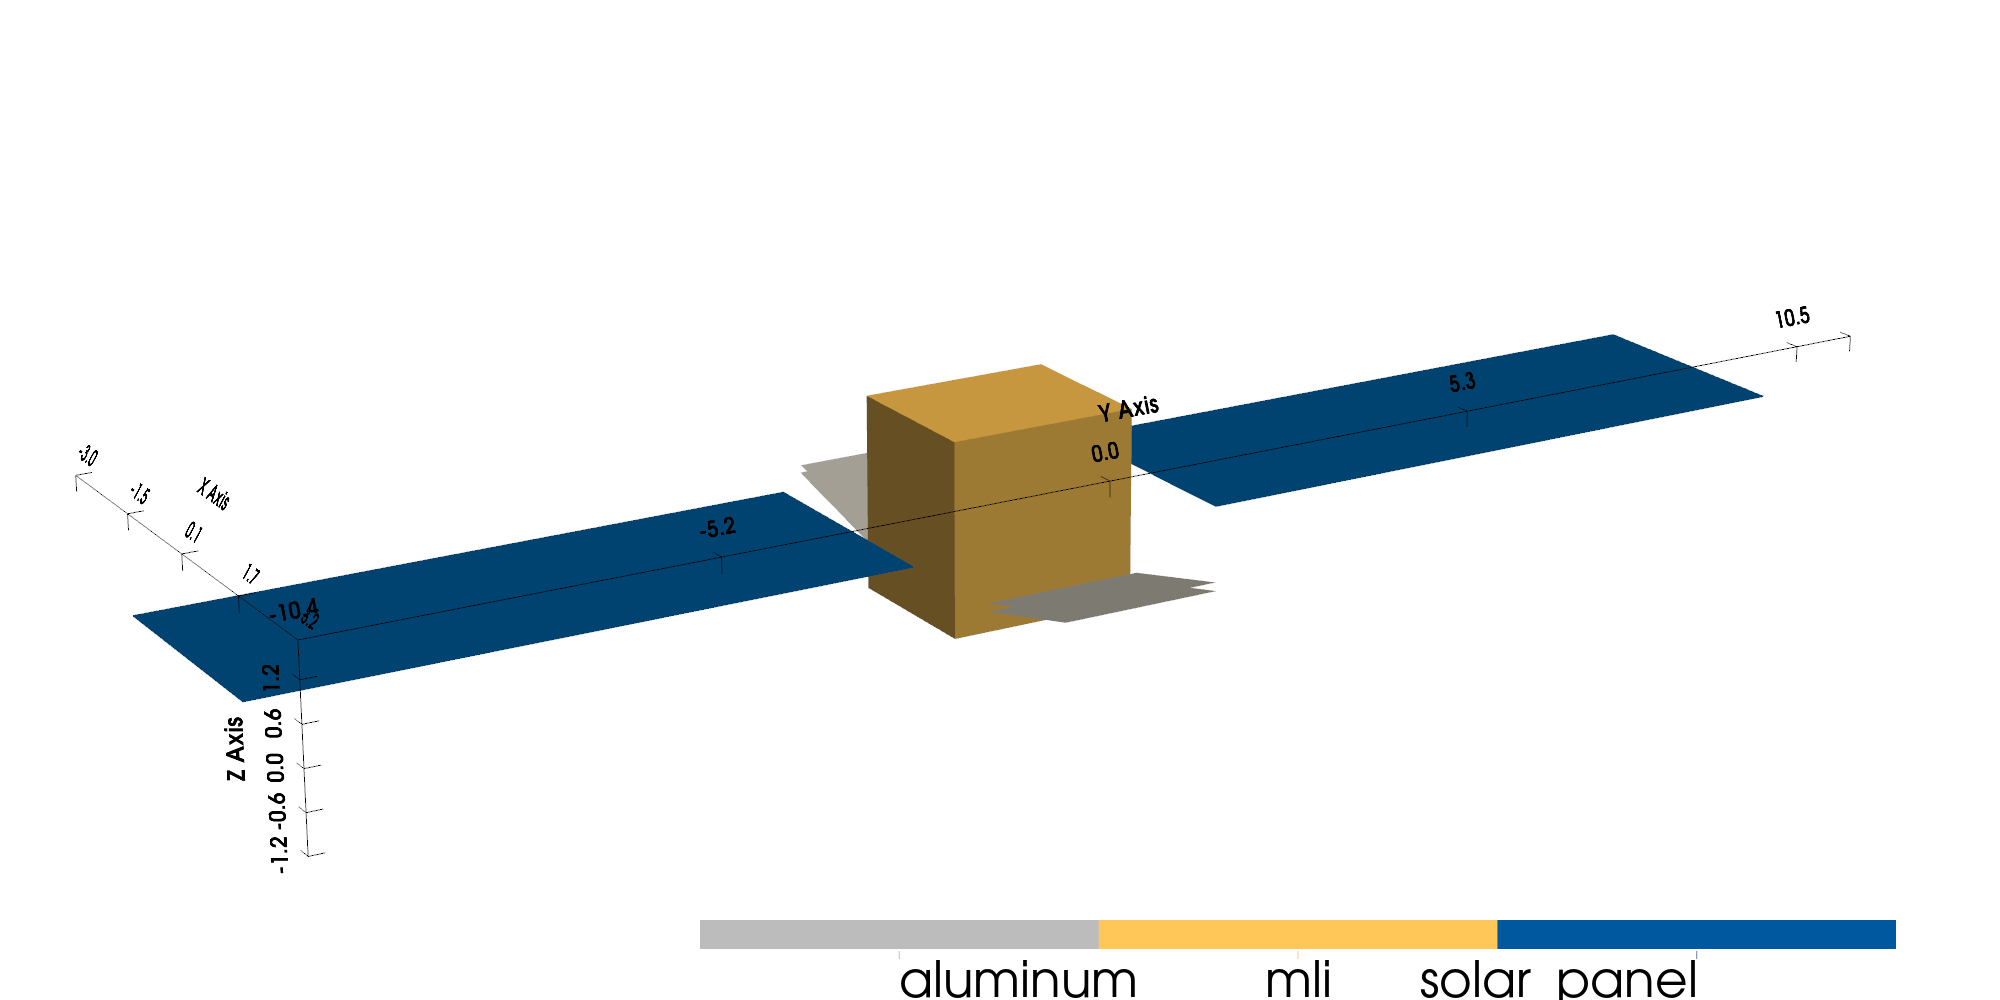
\includegraphics[width=\figbig]{sphx_glr_plot_models_001.png}
  \caption{Simplified ECHOSTAR II box-wing model used for inversion.}
  \label{fig:echostar1_simple}
\end{figure}

The contribution of the bus to the total inertia tensor of ECHOSTAR II is spherically symmetric and given by \cite{satterly1958}:

\begin{align}
 J_\text{bus} &= \frac{1}{6} m_b w_b^2 I_3,
\end{align}

\noindent
assuming that the center of mass (COM) of the bus coincides with the COM of the entire vehicle. By the intermediate axis theorem, the contribution of a panel to the inertia tensor is a function of the displacement of the panel's COM from the vehicle's overall COM $\vctr{r}_p = [ 0, s/2 - l_p/2, 0]^T$:

\begin{equation}
  \begin{split}
 J_\text{pan} = &\frac{m_p}{12} \cdot \text{diag}\left(l_p^2, w_p^2, \left(l_p^2 + w_p^2\right) \right) + \\&m_p \left[ \left( \vctr{r}_p \cdot \vctr{r}_p \right) I_3 - \vctr{r}_p \vctr{r}_p^T \right],
  \end{split}
\end{equation}

\noindent
assuming that the panels have negligible thickness. The overall inertia tensor for ECHOSTAR II is therefore:

\begin{align}
 J_\text{SAT} &= J_\text{bus} + 2J_\text{pan} \\
  &= \text{diag} \left( 9512, 1771, 9609 \right) \: [kg \cdot m^2]
\end{align}

Table \ref{tb:case2_in} summarizes the light curve observations that result in the extracted measurements displayed in Figure \ref{fig:rb_lc_obs}.

\begin{table}[H]
  \centering
  \caption{ECHOSTAR II observation characteristics}
  \vspace*{6pt}
  \begin{tabular}{|l|l|}
  \hline
  \textbf{Variable} & \textbf{Value} \\ \hline
 Target COSPAR ID & 1996-055A \\ \hline
 First obs.\ (UTC) & Feb 26, 2025 04:16:12.279 \\ \hline
 Light curve duration & $19.5$ minutes \\ \hline
 Observations & $456$ ($395$ extracted) \\ \hline
 Obs.\ frequency & $0.388$ Hz \\ \hline
 Integration time & $1$ seconds \\ \hline
  \end{tabular}
  \label{tb:case3_in}
\end{table}

\begin{figure}[H]
  \centering
  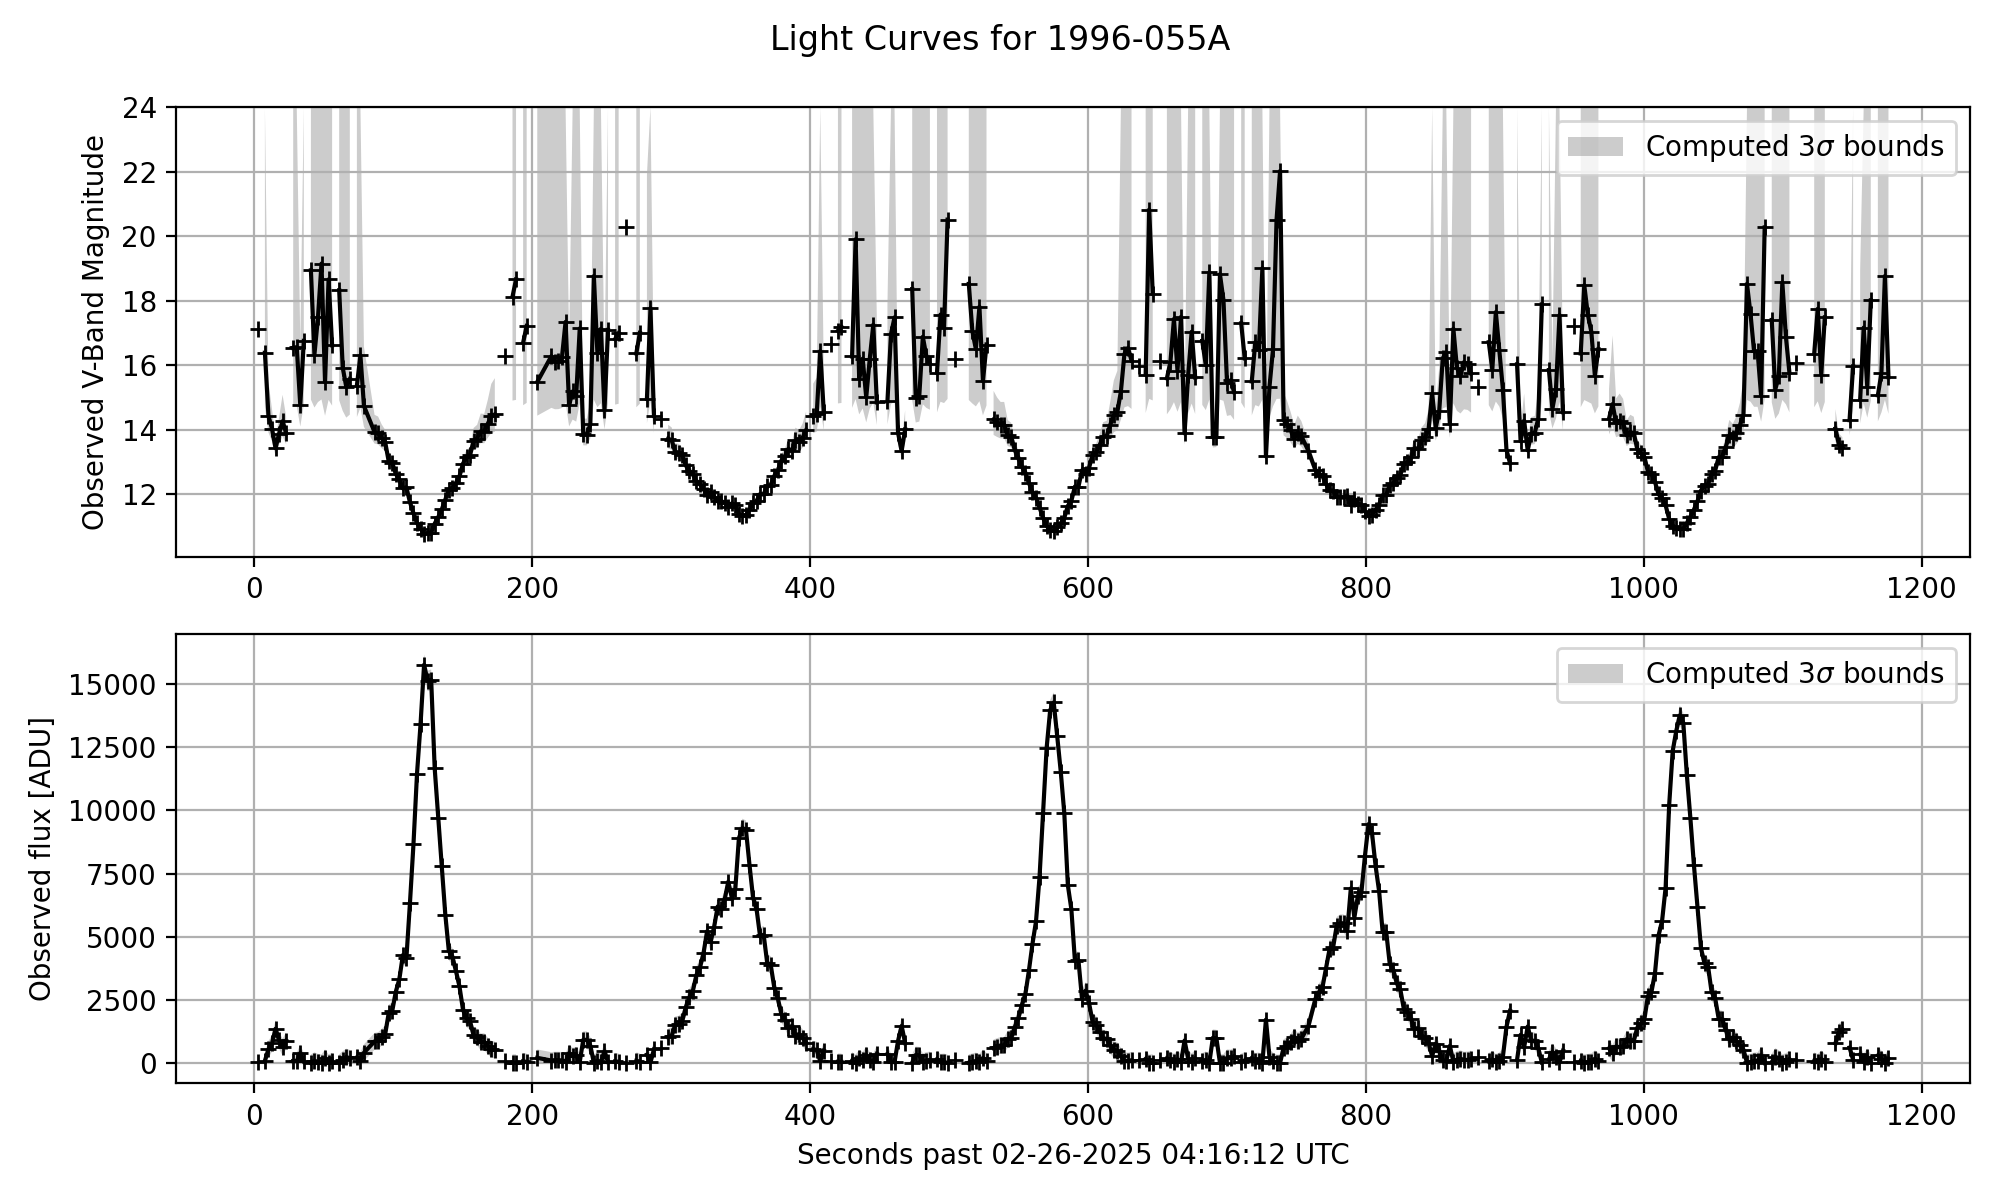
\includegraphics[width=\figbig]{sphx_glr_plot_lcs_002_2_00x.png}
  \caption{Selected light curve for ECHOSTAR II, observed by the Purdue Optical Ground Station}
  \label{fig:sat_lc_obs}
\end{figure}

This light curve is sampled more densely than the Delta I observations, and clearly has significantly more intense specular peaks. Inversion was performed using $10^4$ initial guesses with the material and angular velocity assumptions listed in Table \ref{tb:case3_ass}. The candidate solution results are presented in terms of their mean light curves in Figure \ref{fig:case3_s}, orientation MRPs and angular velocities in Figure \ref{fig:case3_pw}, and inertia ratios in Figure \ref{fig:case3_i}.

\begin{table}[H]
  \centering
  \caption{ECHOSTAR II inversion assumptions}
  \vspace*{6pt}
  \begin{tabular}{|l|l|}
  \hline
  \textbf{Material} & \textbf{Coefficients} \\ \hline
 Aluminum BRDF & $C_d=0.22$, $C_s=0.4$, $n=5$ \\ \hline
 MLI BRDF & $C_d=0.05$, $C_s=0.24$, $n=20$ \\ \hline
 Solar panel BRDF & $C_d=0.05$, $C_s=0.13$, $n=10$ \\ \hline
  $\norm{\vctr{\omega}}_\text{max}$ & $2.32$ $\text{deg} / \text{s}^{-1}$ \\ \hline
  $\ell$ & $1/1000$ \\ \hline
  \end{tabular}
  \label{tb:case3_ass}
\end{table}

\begin{figure*}[t]
  \centering
  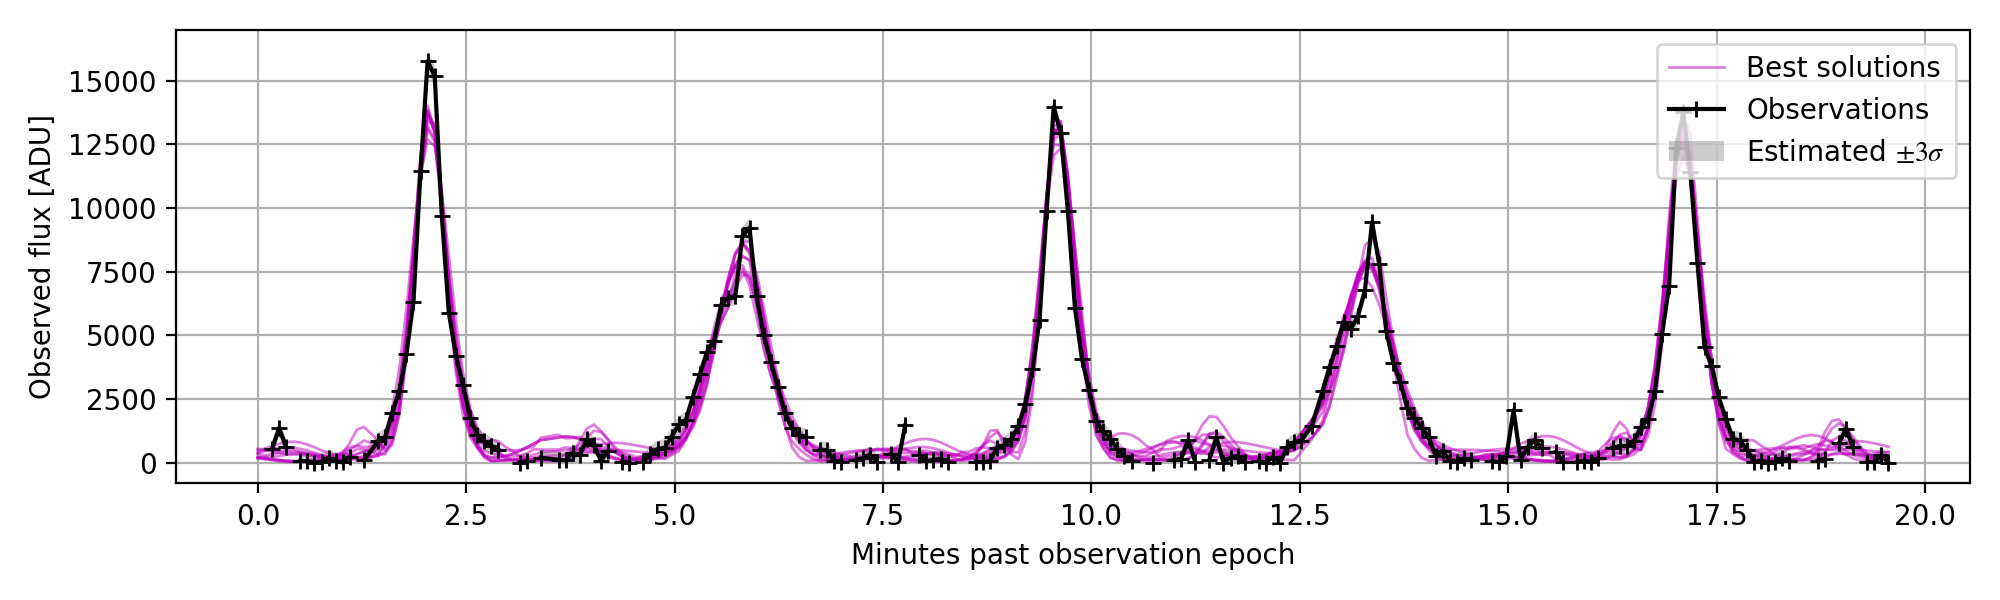
\includegraphics[width=0.8\textwidth]{sphx_glr_results_004_2_00x.png}
  \caption{Candidate solution inertia light curves compared to the real measurements in ADU for ECHOSTAR II.}
  \label{fig:case3_s}
\end{figure*}

\begin{figure}[H]
  \centering
  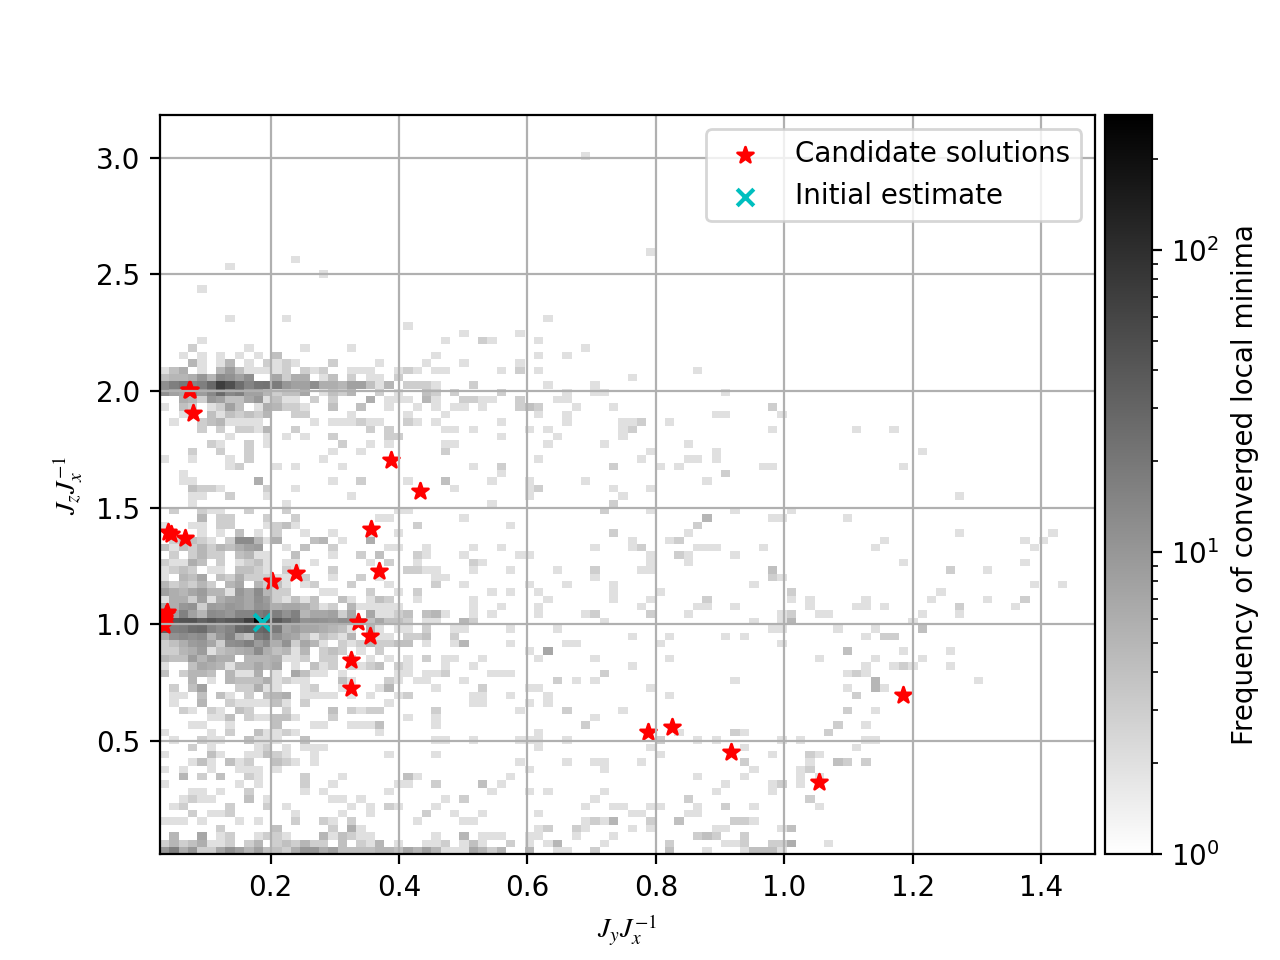
\includegraphics[width=\figmed]{sphx_glr_results_003_2_00x.png}
  \caption{Candidate solution inertia ratio distribution for ECHOSTAR II, non-candidate converged minima are plotted in grey.}
  \label{fig:case3_i}
\end{figure}

\begin{figure}[H]
  \centering
  \begin{subfigure}[t]{0.23\textwidth}
    \centering
    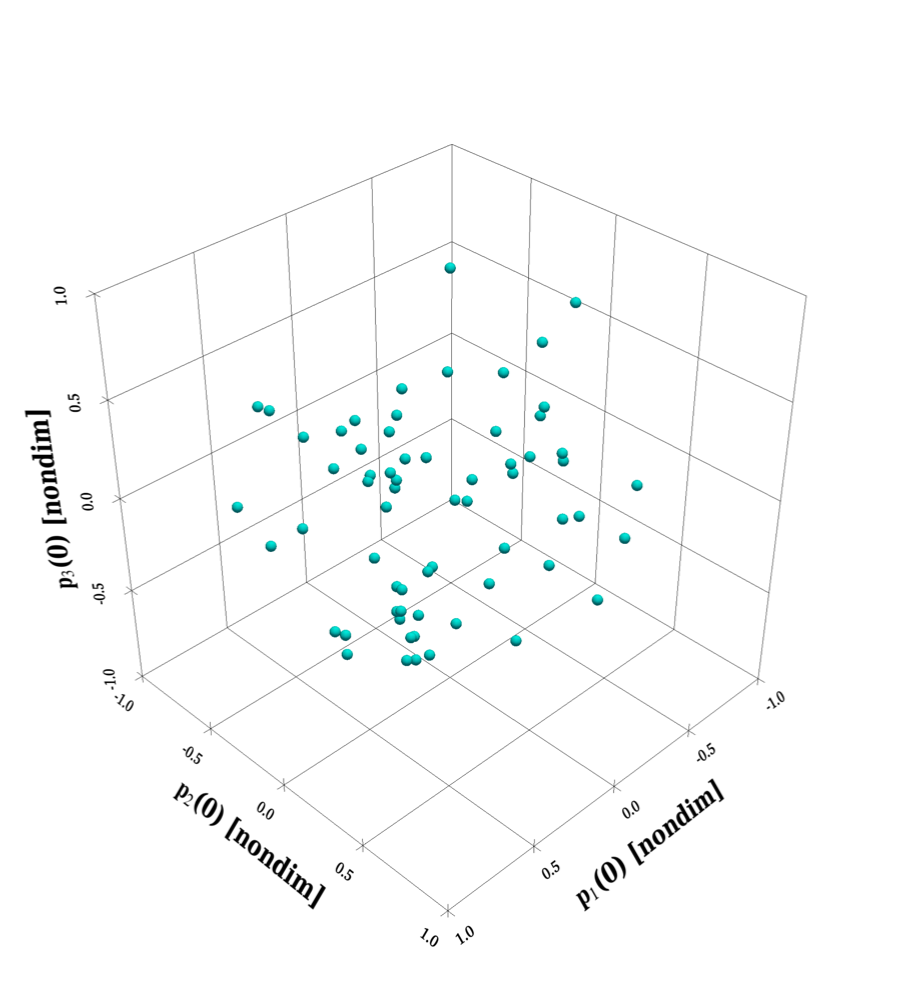
\includegraphics[width=\textwidth]{sphx_glr_results_008.png}
    \caption{MRP}
    \label{fig:case3_pwa}
  \end{subfigure}
  \hfill
  \begin{subfigure}[t]{0.23\textwidth}
    \centering
    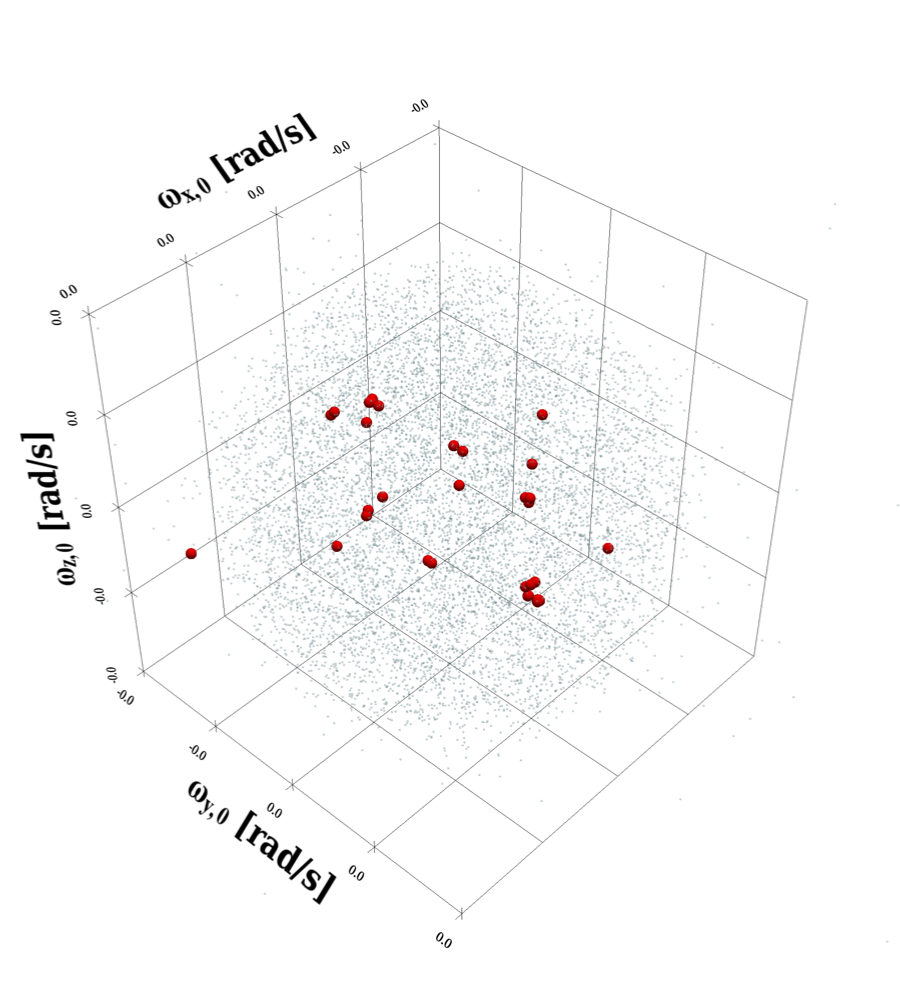
\includegraphics[width=\textwidth]{sphx_glr_results_007.png}
    \caption{Angular velocity}
    \label{fig:case3_pwb}
  \end{subfigure}

  \caption{Candidate solution orientation MRPs and angular velocity vectors for ECHOSTAR II}
  \label{fig:case3_pw}
\end{figure}


% \begin{figure}[H]
%   \centering
%   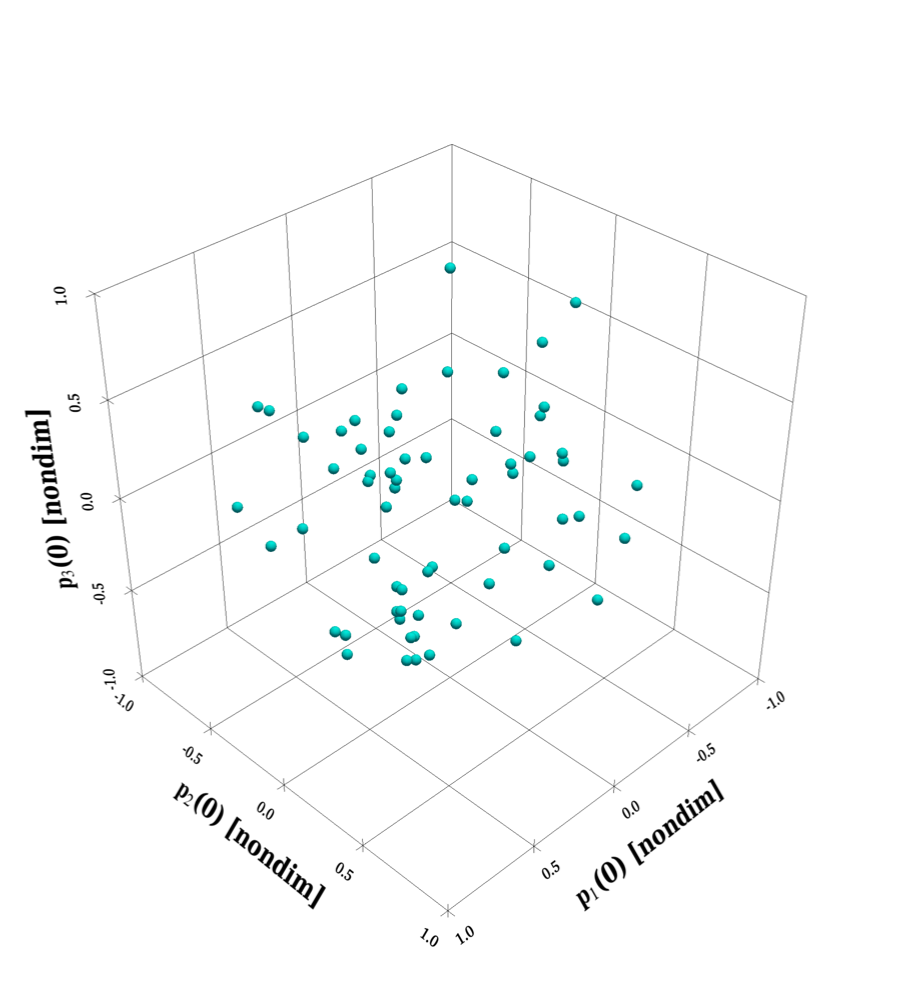
\includegraphics[width=\figmed]{sphx_glr_results_008.png}
%   \caption{Candidate solution orientation MRPs for ECHOSTAR II, non-candidate converged minima are plotted in grey.}
%   \label{fig:case3_p}
% \end{figure}

% \begin{figure}[H]
%   \centering
%   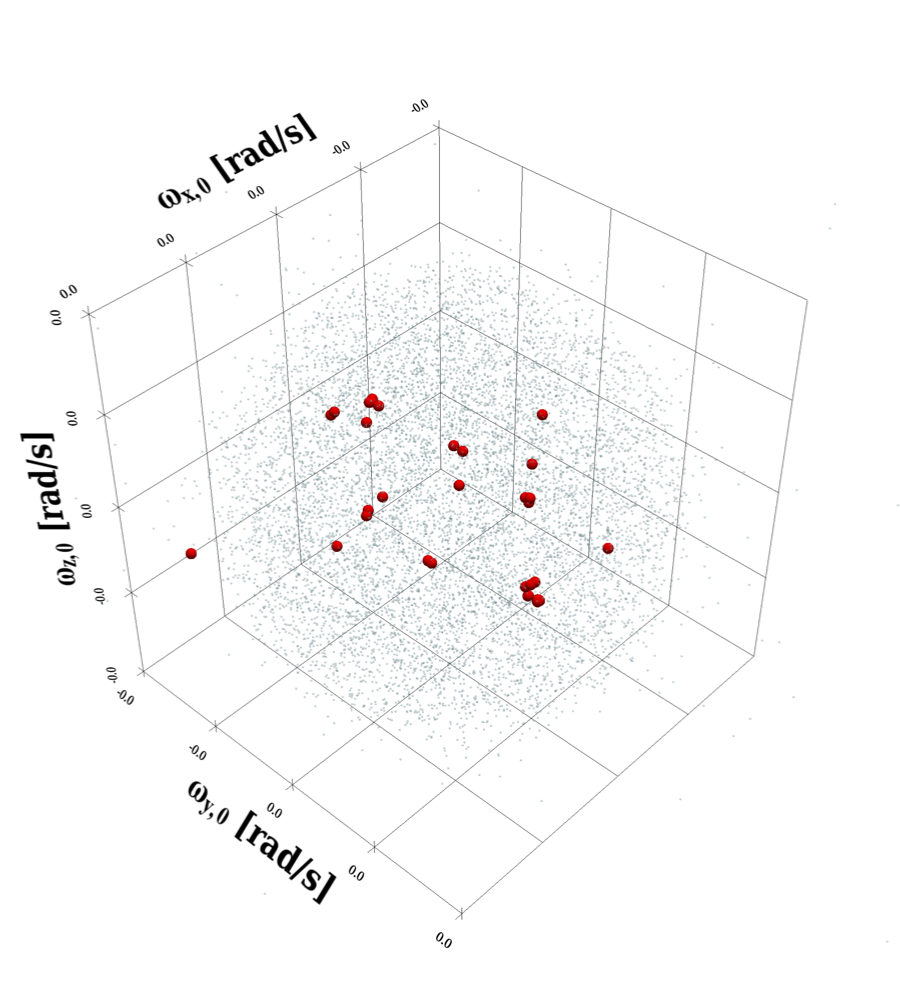
\includegraphics[width=\figmed]{sphx_glr_results_007.png}
%   \caption{Candidate solution angular velocities for ECHOSTAR II, non-candidate converged minima are plotted in grey.}
%   \label{fig:case3_w}
% \end{figure}

The candidate solutions identified by the inversion process are more sparse than those found in either of the previous rocket body cases, with some vague clustering in both angular velocity and orientation space. That said, the candidate light curves fit the data quite well. Notably, the formulation of the negative log-likelihood objective function in Equation \ref{eq:nll_loss} produces the behavior seen in the candidate solutions in Figure \ref{fig:case3_s}, where even the smallest recurrent specular peaks are well-estimated by most solutions. A similar effect -- giving up some of the statistical robustness of our formulation -- can be achieved in an unweighted optimization over the observations in magnitudes. The inertia tensor solutions are dispersed throughout the solution space, with less symmetry than the Delta I solutions. As in the Delta I case, more data about the mass and reflectivity of the object would be necessary to continue refining any of these candidates.

\section{Conclusion}

Attitude information is critical for many tasks informing space situational awareness. Orientation and angular velocity data aids high-fidelity orbit propagation, mission recovery efforts, and object selection for active debris removal. Obtaining attitude information is often difficult, especially for passive debris objects. Due to atmospheric distortion and diffraction-limited optics, ground-based telescopes can only determine a total brightness received from a space object. If a shape model is known, the light curve -- a sequence of these brightness measurements -- is one tool for attitude estimation. We presented an approach for solving this highly nonlinear and non-convex optimization problem with a gradient-based multi-start method. We presented attitude inversion results for one case with synthetic data and two cases with real observations. Unlike other approaches, our method successfully identifies the numerous ambiguous solutions families -- originating from symmetries in the observation geometry and the object shape -- which may produce the same observations. These disparate candidate solutions can serve as starting points for more detailed exploration as additional light curves or further object shape information is obtained.

\section*{Acknowledgments}

This work was partially supported by a National Defense Science and Engineering Graduate Fellowship.

\section*{Appendix}

\begin{table}[H]
  \centering
  \caption{Telescope information for synthetic and real data observations}
  \vspace*{6pt}
  \begin{tabular}{|l|l|}
  \hline
  \textbf{Variable} & \textbf{Value} \\ \hline
 CCD sensor & KAF-16803 \\ \hline
 Effective aperture area $A_\circ$ & $0.076$ $m^2$ \\ \hline
 Observer location & $32.900^\circ \textrm{ N}, -105.533^\circ \textrm{ W}$ \\ \hline
 Observer altitude & $2.24$ km above MSL \\ \hline
 Source pixels $n_\text{pix}$ & $100$ \\ \hline
 Read noise $\sigma_\text{read}$ & $9$ $\text{ADU} / \text{pixel}$ \\ \hline
 Dark current rate $\lambda_\text{dark}$ & $0.01$ $\text{ADU} / \text{pixel} / \text{s}$ \\ \hline
 Flat field strength $f_k$ & $0.01$ nondim \\ \hline
 Gain $g$ & $5.1$ $e^- / \text{ADU}$ \\ \hline
  \end{tabular}
  \label{tb:tele_info}
 \end{table}

 \begin{table}[H]
  \centering
  \caption{BFGS solver configuration for all results cases}
  \vspace*{6pt}
  \begin{tabular}{|l|l|}
  \hline
  \textbf{Variable} & \textbf{Value} \\ \hline
 Maximum function evaluations & $1000$ \\ \hline
 Maximum iterations & $100$ \\ \hline
 Finite difference step size & $1 \cdot 10^{-5}$ \\ \hline
 Gradient $\infty$-norm tolerance & $1 \cdot 10^{-5}$ \\ \hline
  \end{tabular}
  \label{tb:bfgs_info}
 \end{table}

\bibliography{cache/refs.bib}
\end{document}

